% ============================================================
% NetMind - Final Year Project Report (Project 1)
% Prince Sattam Bin Abdulaziz University
%
% Compile with XeLaTeX (needed for the Arabic text):
%     cd latex && latexmk -xelatex main.tex
% or, without latexmk, run `xelatex main.tex` twice.
% On Overleaf: Menu -> Compiler -> XeLaTeX.
% ============================================================
\documentclass[12pt,a4paper,oneside]{report}

% ------------------------------------------------------------
% Fonts and Arabic
% ------------------------------------------------------------
\usepackage{fontspec}
\setmainfont{Liberation Serif}
\setmonofont[Scale=0.92]{Liberation Mono}
% FreeSerif has full Arabic coverage. Any Arabic font works here
% (e.g. Amiri on Overleaf).
\newfontfamily\arabicfont[Script=Arabic,Scale=1.08]{FreeSerif}

% XeTeX's built-in right-to-left typesetting. Used instead of the
% bidi/polyglossia packages so the report also builds on minimal
% TeX installations. Arabic paragraphs are set flush right.
\TeXXeTstate=1
\newenvironment{arabicpar}
  {\par\noindent\arabicfont\leftskip=0pt plus 1fil\rightskip=0pt
   \parfillskip=0pt\beginR}
  {\endR\par}
\newcommand{\ar}[1]{{\arabicfont\beginR #1\endR}}

% ------------------------------------------------------------
% Page layout
% ------------------------------------------------------------
\usepackage[a4paper,left=1in,right=1in,top=1in,bottom=1in]{geometry}
\usepackage{setspace}
\setstretch{1.4}
\setlength{\parskip}{0.55em}
\setlength{\parindent}{0pt}
\usepackage[hyphens]{url}

% ------------------------------------------------------------
% Packages
% ------------------------------------------------------------
\usepackage{graphicx}
\graphicspath{{figures/}}
\usepackage{float}
\usepackage{array}
\usepackage{longtable}
\usepackage{tabularx}
\usepackage{xltabular}
\setlength{\LTpre}{0.6em}\setlength{\LTpost}{0.4em}
\usepackage{enumitem}
\setlist{itemsep=0.25em,topsep=0.3em}
\usepackage[table]{xcolor}
\usepackage{tikz}
\usetikzlibrary{arrows.meta,positioning,fit,calc,shapes.geometric,backgrounds}
\tikzset{every node/.append style={execute at begin node=\setstretch{1.0}}}
\usepackage{caption}
\captionsetup{labelfont=bf,labelsep=colon,font=small,skip=6pt}
\usepackage{titlesec}
\usepackage{tocloft}
\usepackage[hidelinks,unicode]{hyperref}
\hypersetup{
  pdftitle={NetMind: An LLM-Powered Assistant for Network Operations and Security},
  pdfauthor={Khaled Ibrahim Alghmlas, Faleh Hamoud Alsubaie, Ibrahim Abdulrahman Alharthi}
}

% ------------------------------------------------------------
% Colours used in tables and diagrams
% ------------------------------------------------------------
\definecolor{headgray}{gray}{0.88}
\definecolor{boxgray}{gray}{0.96}
\definecolor{userblue}{HTML}{E8EAFB}
\definecolor{guardorange}{HTML}{FCE9D4}
\definecolor{donegreen}{HTML}{1E7B34}
\definecolor{nextred}{HTML}{A61B1B}

% Table helpers: grey header row, wrapped columns
\newcolumntype{L}[1]{>{\raggedright\arraybackslash}p{#1}}
\newcolumntype{Y}{>{\raggedright\arraybackslash}X}
\newcommand{\head}{\rowcolor{headgray}}
\renewcommand{\arraystretch}{1.25}

% ------------------------------------------------------------
% Headings: "CHAPTER 1: INTRODUCTION"
% ------------------------------------------------------------
\titleformat{\chapter}[block]
  {\normalfont\LARGE\bfseries}
  {CHAPTER \thechapter:\ }{0pt}{\MakeUppercase}
\titlespacing*{\chapter}{0pt}{0pt}{1.4em}
\titleformat{\section}{\normalfont\Large\bfseries}{\thesection}{0.6em}{}
\titleformat{\subsection}{\normalfont\large\bfseries}{\thesubsection}{0.6em}{}
\titleformat{\subsubsection}{\normalfont\normalsize\bfseries\itshape}{\thesubsubsection}{0.6em}{}
\setcounter{secnumdepth}{3}
\setcounter{tocdepth}{3}

% Unnumbered front-matter chapters
\newcommand{\frontchapter}[1]{%
  \chapter*{\MakeUppercase{#1}}%
  \addcontentsline{toc}{chapter}{\MakeUppercase{#1}}}

% Small italic run-in heading used inside sections
\newcommand{\para}[1]{\par\medskip\textbf{\textit{#1}}\par}

% Table of contents style
\renewcommand{\cfttoctitlefont}{\normalfont\Huge\bfseries}
\renewcommand{\cftlottitlefont}{\normalfont\Huge\bfseries}
\renewcommand{\cftloftitlefont}{\normalfont\Huge\bfseries}
\renewcommand{\contentsname}{TABLE OF CONTENTS}
\renewcommand{\listtablename}{LIST OF TABLES}
\renewcommand{\listfigurename}{LIST OF FIGURES}
\renewcommand{\cftchapdotsep}{\cftnodots}

% ------------------------------------------------------------
% Shared text
% ------------------------------------------------------------
\newcommand{\projecttitle}{NETMIND: AN LLM-POWERED ASSISTANT FOR NETWORK OPERATIONS AND SECURITY}
% Monospace code; allows a line break after an underscore or a dot
\newcommand{\codeus}{\textunderscore\allowbreak}
\newcommand{\code}[1]{{\ttfamily\let\_\codeus#1}}
\emergencystretch=3em

% ============================================================
\begin{document}
% ============================================================

\pagenumbering{roman}
% ============================================================
% Front matter: cover, title page, declaration, approval,
% acknowledgements, abstracts, lists
% ============================================================

% Team, used on the cover, the title page and the declaration
\newcommand{\teamlist}{%
  Khaled Ibrahim Alghmlas -- 445050235\\
  Faleh Hamoud Alsubaie -- 445050053\\
  Ibrahim Abdulrahman Alharthi -- 445050024}

\newcommand{\titleblock}[1]{% #1 = vertical gap between blocks
  {\LARGE\bfseries\setstretch{1.15}\projecttitle\par}
  \vspace{#1}
  {\large\bfseries\setstretch{1.2}\teamlist\par}
  \vspace{#1}
  To obtain\par
  {\large BSc in Computer Science\par}
  \vspace{0.7\dimexpr#1\relax}
  Department of Computer Sciences\par
  College of Computer Engineering and Sciences\par
  \vspace{0.7\dimexpr#1\relax}
  Supervisor: Dr.\ Khalil Chebil\par
  \vspace{0.7\dimexpr#1\relax}
  December 2026\par}

% ------------------------------------------------------------
% Cover page
% ------------------------------------------------------------
\begin{titlepage}
\setstretch{1.1}
\noindent
\begin{minipage}[b]{0.4\textwidth}
\footnotesize
Kingdom of Saudi Arabia\\
Ministry of Education\\
Prince Sattam Bin Abdulaziz University\\
College of Computer Engineering and Sciences\\
Department of Computer Sciences
\end{minipage}\hfill
\begin{minipage}[b]{0.2\textwidth}
\centering
\includegraphics[width=0.75\linewidth]{psau-logo.jpeg}
\end{minipage}\hfill
\begin{minipage}[b]{0.36\textwidth}
\raggedleft\footnotesize
\ar{المملكة العربية السعودية}\\
\ar{وزارة التعليم}\\
\ar{جامعة الأمير سطام بن عبد العزيز}\\
\ar{كلية هندسة وعلوم الحاسب}\\
\ar{قسم علوم الحاسب}
\end{minipage}

\vspace{1.6cm}
\begin{center}
\titleblock{1.2cm}
\vspace{0.6cm}
Number: *****
\end{center}
\end{titlepage}

% ------------------------------------------------------------
% Title page
% ------------------------------------------------------------
\begin{titlepage}
\vspace*{2.5cm}
\begin{center}
\titleblock{1.8cm}
\end{center}
\end{titlepage}

% ------------------------------------------------------------
% Declaration
% ------------------------------------------------------------
\setcounter{page}{2}
\frontchapter{Declaration}

I/we hereby declare that this project report is based on my/our original
work except for citations and quotations which have been duly acknowledged.
I/We also declare that it has not been previously or concurrently submitted
for any other degree at PSAU or any other institution.

\vspace{1.5cm}
\noindent Signature:\ \dotfill\ \ \ Date:\ \makebox[5cm]{\dotfill}

\vspace{1cm}
\noindent
\begin{tabular}{@{}p{0.5\textwidth}l@{}}
Name: Khaled Ibrahim Alghmlas      & ID: 445050235 \\[0.4em]
Name: Faleh Hamoud Alsubaie        & ID: 445050053 \\[0.4em]
Name: Ibrahim Abdulrahman Alharthi & ID: 445050024 \\
\end{tabular}

% ------------------------------------------------------------
% Approval
% ------------------------------------------------------------
\frontchapter{Approval for Submission}

I certify that this project report entitled \textbf{``\projecttitle''} was
prepared by Khaled Ibrahim Alghmlas, Faleh Hamoud Alsubaie and Ibrahim
Abdulrahman Alharthi and has met the required standard for submission in
partial fulfillment of the requirements for the degree of Bachelor of Science
in Computer Science at PSAU.

\vspace{1.2cm}
Approved by

\vspace{2cm}
\noindent Signature:\ \makebox[7cm]{\dotfill}

\noindent Supervisor: Dr.\ Khalil Chebil

\noindent Date:\ \makebox[7cm]{\dotfill}

% ------------------------------------------------------------
% Acknowledgements
% ------------------------------------------------------------
\frontchapter{Acknowledgements}

We would like to express our sincere gratitude to our supervisor,
Dr.\ Khalil Chebil, for his continuous guidance, encouragement, and valuable
feedback throughout the course of this project, including his encouragement
to begin early development work ahead of schedule and the detailed
improvement plan he prepared for the system. We are also grateful to the
faculty members of the Department of Computer Sciences at Prince Sattam Bin
Abdulaziz University for the knowledge and support that made this project
possible.

We would like to thank each other as a team: Khaled Ibrahim Alghmlas, Faleh
Hamoud Alsubaie and Ibrahim Abdulrahman Alharthi, for the collaboration and
shared effort that went into every part of NetMind. We would also like to
thank our fellow students working on other graduation projects who generously
shared their insights and discussed ideas with us on topics related to this
work.

% ------------------------------------------------------------
% Abstract (English)
% ------------------------------------------------------------
\frontchapter{Abstract}

\begin{center}
\textbf{\projecttitle}
\end{center}

Modern networks combine many types of devices --- routers, switches,
firewalls, and IoT equipment such as IP cameras --- and administering them
typically requires familiarity with several vendor-specific command-line
interfaces, which slows operations and increases the risk of operator error.
This project presents NetMind, a network operations assistant that lets a
user manage and monitor a network through natural-language conversation in
Arabic or English rather than memorised commands. NetMind is built around a
Large Language Model, accessed through the Groq API, given callable tools to
check device status and IP addresses, power devices on or off, list devices
on a network segment, test connectivity between devices, audit a firewall's
configuration for common weaknesses, and verify whether a security camera
still uses its default password. Destructive actions are never executed on
the model's word alone: they require explicit confirmation by the user in the
interface and are recorded in an audit log.

To allow safe experimentation, NetMind operates against a simulated network
built with Containerlab, with real IP addressing and routing between
branches, so every action is executed against a genuine, contained network
rather than a mock. A second, read-only mode extends the same interface to a
real physical network, discovering devices by combining ARP scanning, a ping
sweep, IPv6 neighbour discovery and mDNS without altering their state. A
working prototype of both modes, together with a live monitoring dashboard,
alert notifications, persistent storage and an automated test suite, was
built and validated ahead of schedule. This document covers the motivation,
requirements, design, and architecture of NetMind, the reasoning behind the
tools and techniques chosen to build it, and the plan for the second term.

% ------------------------------------------------------------
% Abstract (Arabic)
% ------------------------------------------------------------
\chapter*{\hfill\ar{المستخلص}}
\addcontentsline{toc}{chapter}{ABSTRACT (ARABIC)}

\begin{center}
\ar{\textbf{نتمايند: مساعد قائم على نماذج اللغة الكبيرة لإدارة وتأمين الشبكات}}
\end{center}

\begin{arabicpar}
تجمع الشبكات الحديثة أنواعًا عديدة من الأجهزة، مثل الموجهات والمحولات
(السويتشات) وجدران الحماية ومعدات إنترنت الأشياء كالكاميرات الأمنية،
وعادةً ما تتطلب إدارتها الإلمام بعدة واجهات أوامر نصية خاصة بكل مورّد، مما
يُبطئ عمليات التشغيل ويزيد من احتمال وقوع أخطاء بشرية. يقدّم هذا المشروع
نظام نتمايند (NetMind)، وهو مساعد لعمليات الشبكات يتيح للمستخدم إدارة
الشبكة ومراقبتها من خلال محادثة بلغة طبيعية باللغتين العربية والإنجليزية،
بدلاً من حفظ الأوامر. يعتمد نتمايند على نموذج لغوي كبير، يُستدعى عبر واجهة
Groq البرمجية، زُوّد بمجموعة من الأدوات القابلة للاستدعاء للتحقق من حالة
الأجهزة وعناوين IP الخاصة بها، وتشغيلها أو إيقافها، وسرد الأجهزة على جزء
معيّن من الشبكة، واختبار الاتصال بين الأجهزة، وتدقيق إعدادات جدار الحماية
للكشف عن الثغرات الشائعة، والتحقق مما إذا كانت كاميرا المراقبة ما زالت
تستخدم كلمة المرور الافتراضية. ولا تُنفَّذ الإجراءات التدميرية بناءً على
كلام النموذج وحده، بل تتطلب تأكيدًا صريحًا من المستخدم في الواجهة وتُسجَّل
في سجل تدقيق.
\end{arabicpar}

\begin{arabicpar}
ولإتاحة التجربة الآمنة، يعمل نتمايند على شبكة محاكاة مبنية باستخدام
Containerlab، بعنونة IP وتوجيه حقيقيين بين الفروع، بحيث يُنفَّذ كل إجراء
على شبكة حقيقية ومحتواة فعلاً وليس على نموذج وهمي. كما يوفر النظام وضعًا
ثانيًا للقراءة فقط يمتد بالواجهة نفسها إلى شبكة فعلية حقيقية، حيث يكتشف
الأجهزة المتصلة بالجمع بين فحص ARP وفحص ping واكتشاف جيران IPv6 وبروتوكول
mDNS دون التأثير في حالتها. وقد تم بناء نموذج أولي يُطبّق كلا الوضعين، إلى
جانب لوحة مراقبة حيّة وتنبيهات وتخزين دائم ومجموعة اختبارات آلية، والتحقق من
عمله قبل الموعد المقرر. ويغطي هذا التقرير دوافع المشروع ومتطلباته وتصميمه
ومعماريته، والأسباب وراء اختيار الأدوات والتقنيات المستخدمة في بنائه، وخطة
العمل للفصل الدراسي الثاني.
\end{arabicpar}

% ------------------------------------------------------------
% Lists
% ------------------------------------------------------------
\cleardoublepage
\tableofcontents
\cleardoublepage
\listoftables
\cleardoublepage
\listoffigures

% ------------------------------------------------------------
% Abbreviations
% ------------------------------------------------------------
\frontchapter{List of Symbols/Abbreviations}

\setlength{\LTleft}{0pt}
\begin{longtable}{@{}p{3.2cm}l@{}}
AI      & Artificial Intelligence \\
API     & Application Programming Interface \\
ARP     & Address Resolution Protocol \\
CI      & Continuous Integration \\
CPU     & Central Processing Unit \\
CVE     & Common Vulnerabilities and Exposures \\
DHCP    & Dynamic Host Configuration Protocol \\
DNS     & Domain Name System \\
FR      & Functional Requirement \\
HTTP    & Hypertext Transfer Protocol \\
ICMP    & Internet Control Message Protocol \\
IoT     & Internet of Things \\
IP      & Internet Protocol \\
JSON    & JavaScript Object Notation \\
LLM     & Large Language Model \\
MAC     & Media Access Control \\
MCP     & Model Context Protocol \\
mDNS    & Multicast Domain Name System \\
NDP     & Neighbor Discovery Protocol (IPv6) \\
NETCONF & Network Configuration Protocol \\
NFR     & Non-Functional Requirement \\
OUI     & Organizationally Unique Identifier \\
OWASP   & Open Worldwide Application Security Project \\
PSAU    & Prince Sattam Bin Abdulaziz University \\
RBAC    & Role-Based Access Control \\
REST    & Representational State Transfer \\
SDK     & Software Development Kit \\
SNMP    & Simple Network Management Protocol \\
SQL     & Structured Query Language \\
SSDP    & Simple Service Discovery Protocol \\
SSH     & Secure Shell \\
TCP     & Transmission Control Protocol \\
UDP     & User Datagram Protocol \\
UPnP    & Universal Plug and Play \\
VM      & Virtual Machine \\
WSL     & Windows Subsystem for Linux \\
YAML    & YAML Ain't Markup Language \\
\end{longtable}

% ------------------------------------------------------------
% Keywords
% ------------------------------------------------------------
\frontchapter{List of Keywords}

NetMind, Large Language Models, Network Automation, Network Security,
Containerlab, Firewall Auditing, Network Simulation, Natural Language
Interface, Docker, Network Operations, Tool Calling, AI Agent, Network
Discovery, Network Topology, Python, Scapy, SQLite.


\cleardoublepage
\pagenumbering{arabic}
% ============================================================
\chapter{Introduction}
% ============================================================

\section{Purpose of the Project}

Modern computer networks combine a wide range of devices, including routers,
switches, firewalls, and Internet of Things equipment such as IP cameras.
Administering and monitoring these devices normally requires operators to be
familiar with several vendor-specific command-line interfaces, which makes
network operations slow, error-prone, and difficult for less experienced
staff to perform safely.

The purpose of this project is to design and implement NetMind, a network
operations assistant that allows a user to manage and monitor a network using
natural language instead of memorised commands. NetMind is built around a
Large Language Model, accessed through the Groq API, which is given a set of
callable tools that can check a device's power state and IP address, turn
devices on or off, list every device on a given network segment, test whether
two devices can reach each other, audit a firewall's configuration for common
security weaknesses such as an open SSH port, and verify whether a security
camera is still using its default password. The system understands requests
in both Arabic and English and responds through a web application that
combines the chat with a live monitoring dashboard.

To allow safe experimentation, NetMind operates in a simulated mode against a
virtual network built with Containerlab, consisting of a router, firewalls,
switch and hub segments, hosts, and cameras running inside Docker containers
with real IP addressing and routing between branches. A second, read-only
real-network mode extends the same natural-language interface to an actual
physical network, discovering connected devices by combining ARP scanning, a
ping sweep, IPv6 neighbour discovery and mDNS. Together, these two modes
demonstrate that a single conversational interface can be used both to learn
and test network administration safely, and to observe a real network
without requiring the user to run separate diagnostic tools.

\section{Purpose of this Document}

This document is prepared in partial fulfilment of the requirements for the
degree of Bachelor of Science in Computer Science at the College of Computer
Engineering and Sciences, Prince Sattam Bin Abdulaziz University. It records
the motivation behind NetMind, the analysis and design decisions taken while
building it, the implementation of its simulated and real-network modes, the
testing carried out to confirm that the system behaves correctly and safely,
and the plan for the second term of the project.

The primary readers of this document are the project supervisor,
Dr.\ Khalil Chebil, and the examining committee responsible for assessing
this Final Year Project. It is also intended to be useful to any student or
developer who wishes to understand, maintain, or extend NetMind in the
future, by explaining not only what was built but why particular design
choices were made.

\section{Overview of this Document}

The remainder of this document is organised as follows.

Chapter~2, Literature Review, examines existing approaches to network
management and related tools, and positions NetMind relative to them.

Chapter~3, System Analysis, presents the requirements gathered for the
project, including functional and non-functional requirements, together with
a diagram describing how a user interacts with the system.

Chapter~4, Design Considerations, discusses the constraints that shaped the
project, the hardware and software environment used, and the development
method followed.

Chapter~5, System Design, describes the architecture of NetMind in detail:
its layered structure, the device registry and services, the tool registry
that connects them to the Large Language Model, the simulated Containerlab
network, the real-network discovery mode and the live monitoring dashboard,
together with its confirmation and audit safeguards, its persistent storage,
and the testing carried out.

Chapter~6, Conclusion, summarises what was achieved, reflects on the
limitations of the current system, and sets out the work planned for the
second term, followed by the References and Appendices.

% ============================================================
\chapter{Literature Review}
% ============================================================

\section{Review of Literature}

\para{Traditional Network Management}

Network management has long relied on standard protocols rather than on
natural language. The Simple Network Management Protocol (SNMP) lets a
management station read and change variables on routers, switches and other
devices (Case et al., 1990), and its later architecture added security and
extensibility to the same model (Harrington et al., 2002). NETCONF replaced
much of SNMP's configuration role with a structured, transaction-based
protocol for installing and changing device configuration (Enns et al.,
2011). These protocols made automation possible, but they expose low-level
data models: an operator, or a script written by one, must still know
exactly which variable or configuration element to read or change.

Intent-Based Networking (IBN) is the research community's response to this
gap. RFC~9315 defines intent as a statement of the outcome an operator
wants, rather than the steps to reach it, and describes systems that
translate such intent into configuration and then check that it is being met
(Clemm et al., 2022). The same document notes that intent-based networking is
a natural candidate for artificial intelligence techniques. LLMs offer a
practical way to express intent in everyday language, which is the approach
NetMind takes.

\para{Language Models That Use Tools}

NetMind depends on an LLM being able to act, not only to answer. Yao et al.\
(2023) showed with ReAct that interleaving reasoning steps with actions such
as calls to external tools makes language models more accurate and their
behaviour easier to inspect, and Schick et al.\ (2023) showed with Toolformer
that a model can learn when and how to call external interfaces on its own.
Modern LLM APIs expose this ability as \emph{function calling} or \emph{tool
calling}, which NetMind uses: the model chooses a tool and its arguments,
and NetMind's own code decides whether and how to run it.

\para{LLMs for Network Management}

Research on applying large language models (LLMs) to network management has
grown rapidly since 2023. Hong, Van Tu, and Hong (2025) provide a
comprehensive survey of this field, classifying LLM-based approaches into
five task areas: network design, configuration, fault management, security,
and orchestration. Their analysis shows that most existing studies address
only one stage of the management workflow in isolation, rely on simulated or
historical data rather than live infrastructure, and still suffer from
hallucination and limited reliability when scaled to complex, heterogeneous
environments.

At the systems level, Wang et al.\ (2025) describe Confucius, a multi-agent
LLM framework developed at Meta that models network management workflows as
directed acyclic graphs and coordinates several specialised agents, each
responsible for a distinct sub-task, to carry out complex operator intents
while validating actions before execution. This illustrates one architectural
direction for LLM-based network management: decomposing a task among
cooperating agents rather than relying on a single general-purpose model.

Closer to the security-focused component of NetMind, Jiang, Gember-Jacobson,
and Feamster (2024) propose CAIP, a framework that supplies LLMs with
carefully mined network-specific context to detect router misconfigurations,
reporting a full detection rate on synthetic faults and the discovery of
previously unnoticed issues in real configurations. Lorusso, Maci, and Coscia
(2025) propose GOLLUM, a conversational agent that guides firewall
configuration using a retrieval-augmented LLM to compensate for the limited
domain-specific knowledge of general-purpose models. Both studies confirm that
LLMs can meaningfully assist with network security tasks when given the right
supporting context, but each addresses a single, narrow task rather than an
integrated management platform.

\para{AI on Both Sides of Security}

The same abilities are changing cybersecurity in both directions. A
systematic review of 185 studies on LLMs for cybersecurity identifies
LLM-based autonomous agents as a significant emerging trend, moving from
single tasks to orchestrating complex, multi-step security workflows (Xu et
al., 2024). On the attacking side, Fang et al.\ (2024) showed that a single
LLM agent given tools and a vulnerability description could autonomously
exploit 87\% of a benchmark of 15 real-world one-day vulnerabilities, where
open-source vulnerability scanners exploited none. The incidents described
in Chapter~1, the agent-driven intrusion at Hugging Face and the AI-assisted
PHP2Shell exploits, show that this is no longer only a laboratory result.
Defenders therefore need tools that work at a comparable speed, but because
a wrong change to a network can itself cause an outage, those tools must
keep a human in control of every change. This balance is the design goal of
NetMind.

\section{Brief Description of Existing Systems}

Beyond academic studies, network management is supported by established
monitoring tools and, more recently, by LLM-based assistants offered as
commercial products and independent open-source projects.

Nagios (Nagios Enterprises, n.d.) and Zabbix (Zabbix LLC, n.d.) are widely
used open-source monitoring systems. They poll devices and services, often
over SNMP, show their state on dashboards, and raise alerts when a check
fails or a threshold is crossed. They are mature and scale to large networks,
but each check, threshold and alert must be configured by an expert, they
have no natural-language interface, and acting on an alert still means
returning to the command line.

Selector AI Copilot (Selector AI, n.d.) is a commercial platform that
grounds an LLM in real network telemetry, allowing operators to ask natural-language questions about
their infrastructure and, through an agent framework, translate the answers
into automated operational workflows.

JACE (ntunes, n.d.) is an open-source autonomous agent that connects to
real Junos network devices over SSH and NETCONF, performs scheduled health checks, detects
anomalies, and answers natural-language questions about the network, while
retaining memory of device state and past incidents across sessions.

The two LLM-based systems represent, respectively, an enterprise-grade
commercial product and an independently developed open-source project, both
operating exclusively against real production networks.

\section{Advantages and Disadvantages of Existing Systems}

The systems reviewed above demonstrate clear strengths. Traditional
monitoring tools such as Nagios and Zabbix are proven, free to use and
reliable at scale, and they detect problems without anyone having to ask.
Selector AI benefits
from mature integration with real telemetry sources and an established agent
framework suited to production environments. JACE benefits from persistent
memory across sessions, allowing it to correlate incidents and remember
device baselines over time, and from directly automating monitoring without
requiring an operator to ask. CAIP and GOLLUM demonstrate that narrowly scoped
LLM systems can achieve very high accuracy within their specific task, since
focusing on one problem allows deeper, more reliable context engineering.

These strengths come with trade-offs. Selector AI is designed for large, real
production networks and offers no safe environment in which students or new
operators can experiment without risk to a live network. JACE, and most of
the studies surveyed by Hong et al.\ (2025), operate only against real
devices, so an operational mistake by the LLM or the operator directly affects
real infrastructure; none of them provide an isolated simulated environment
for safe testing. CAIP and GOLLUM are limited to a single task,
misconfiguration detection or firewall configuration respectively, and do not
extend to device control, monitoring, or other management functions, so they
would need to be combined with other tools to form a complete management
platform.

There is no system among those reviewed that combines a safe testing
environment with broad, integrated functionality while remaining open source.

\section{Problems with Existing Systems}

Drawing on the systems above, four recurring problems can be identified.
The first three concern current LLM-based network management tools. First, most systems that act on
real infrastructure provide no safe, isolated environment in which an LLM's
actions can be tested before being trusted, which is a significant barrier for
an educational or early-stage project where mistakes must be recoverable.
Second, systems that do provide broad functionality, such as Confucius,
achieve this through complex multi-agent orchestration, which increases
engineering effort and is difficult to replicate at a smaller scale. Third,
task-specific systems such as CAIP and GOLLUM achieve strong results within
their domain but do not generalise to device control, network visibility, or
camera and endpoint security, leaving a gap between narrow, highly accurate
tools and broad, general-purpose but less specialised ones. Fourth,
traditional monitoring tools report problems well but cannot be asked
questions in everyday language and do not help the operator act on what
they find, which keeps the cognitive load described in Chapter~1 on the
operator.

{\small
\begin{xltabular}{\textwidth}{|L{3.3cm}|L{2.7cm}|Y|L{2.1cm}|L{1.7cm}|}
\hline
\head \textbf{System (type)} & \textbf{Safe testing environment} & \textbf{Task scope} & \textbf{Natural language} & \textbf{Open source} \\ \hline
\endhead
Nagios / Zabbix (traditional monitoring) & No: monitors live networks & Broad: polling, dashboards and threshold alerts & No & Yes \\ \hline
Selector AI Copilot (commercial AIOps platform) & No: live production networks only & Broad: observability and agent workflows & Yes & No: commercial \\ \hline
JACE (open-source agent for Junos) & No: real devices over SSH / NETCONF & Broad: health checks, anomalies, Q\&A & Yes & Yes \\ \hline
CAIP (research prototype) & N/A: research only & Narrow: router misconfiguration detection & No: LLM used internally & Partial \\ \hline
GOLLUM (research prototype) & N/A: research only & Narrow: firewall configuration & Yes & Partial \\ \hline
Confucius (multi-agent LLM framework) & No & Broad but complex: multi-agent orchestration & Yes (operator intents) & No \\ \hline
\textbf{NetMind (this project)} & \textbf{Yes: simulated lab and read-only real mode} & \textbf{Broad: twenty-one tools for devices, firewalls, cameras, diagnostics and discovery} & \textbf{Yes: Arabic and English} & \textbf{Yes: on GitHub} \\ \hline
\caption{Comparison of NetMind with existing systems}\label{tab:comparison}\\
\end{xltabular}}

\section{Proposed System}

NetMind addresses these problems directly. It pairs a fully simulated
Containerlab network, in which every device is a real, independently
controllable Docker container, with a strictly read-only real-network
discovery mode, so that destructive or exploratory actions by the LLM are
confined to a disposable simulated environment while the real network can
only ever be observed. The boundary is enforced in code: the real-network
backend simply has no capability to change a device, whatever the model
asks. This removes the safety concern identified in existing
real-network-only tools such as Selector AI and JACE. Rather than a
multi-agent architecture, NetMind uses a single language model with a
defined set of callable tools spanning device control, network visibility,
connectivity checks, firewall auditing, and camera security, which keeps the
system simpler to build and reason about than a framework like Confucius
while still covering more ground than single-task systems such as CAIP or
GOLLUM. Each conversation is paired with a live dashboard and an alert
history that reflect the current state of the network, so that every query
is answered from up-to-date system state rather than from potentially stale
conversational memory. Unlike traditional monitoring tools, the same
conversation that reports a problem can also, after the operator confirms,
act on it.

\section{Alternative Solutions Considered}

\para{Network Simulation Platform}

Several network simulation platforms were evaluated before choosing
Containerlab for NetMind's simulated network. Cisco Packet Tracer is widely
used for teaching, but its nodes are not real operating systems and cannot be
controlled programmatically from outside the application. GNS3 and EVE-NG run
real device images, but typically inside full virtual machines, which is
heavier on resources and oriented toward a graphical, VM-centric workflow.
Mininet is lightweight and Python-based, but its network model is built
around virtual switches for software-defined-networking research rather than
independently controllable general-purpose containers. Kathara is
Docker-based, similar in spirit to Containerlab, but has a smaller ecosystem
and less adoption in real network-engineering contexts. Containerlab was
chosen because each node it creates is a real, independently addressable
Docker container: NetMind's control layer can use the standard Docker SDK to
start, stop, and execute commands inside any device exactly as on a real
Linux host, including running iptables on the firewalls and a small HTTP
service on the cameras, a level of direct, programmatic, container-native
control that none of the other evaluated tools offered.

\para{Large Language Model Provider}

Several ways of providing the language model behind NetMind were also
considered. The OpenAI and Anthropic APIs offer strong general-purpose models
with mature tool-calling support, but at higher per-token latency and cost
than were necessary for this project. A locally self-hosted model, for
example through Ollama, would avoid ongoing API costs, but requires capable
local hardware to run reliably enough for consistent tool-calling and
bilingual Arabic/English understanding, which was not practical in the
project's development environment. Groq was chosen because it exposes an
OpenAI-compatible tool-calling interface while running open-weight models
such as \code{openai/gpt-oss-120b} on inference hardware built specifically
for low response latency. Since NetMind's agent loop can make several
sequential tool calls to satisfy a single user request, per-call latency
compounds directly into the user's perceived response time, making Groq's
inference speed a directly relevant advantage rather than an incidental one.
The model is reached through a small provider interface (Section~5.2.3), so
this choice can be revisited without changing the rest of the system.

% ============================================================
\chapter{System Analysis}
% ============================================================

\section{Data Flow Diagrams / Use Case Diagrams}

NetMind exposes a single actor, the User, who interacts with the system
entirely through one web application rather than a set of separate tools or
commands. Figure~\ref{fig:usecase} shows the use cases reachable from that
entry point, grouped by the mode active at the time of the request. Every use
case in Simulated Mode can change the state of the lab network, while every
use case in Real Network Mode is read-only by design, reflecting the safety
boundary described in Chapter~5: the real-network backend has no capability
that could alter a device outside the Containerlab lab, regardless of how a
request is phrased. Within Simulated Mode, the use cases that change state in
a way that is hard to undo (powering a device off, blocking or allowing a
port, changing a camera's credentials) additionally require the user's
explicit confirmation before they run (Section~\ref{sec:guard}).

\begin{figure}[H]
\centering
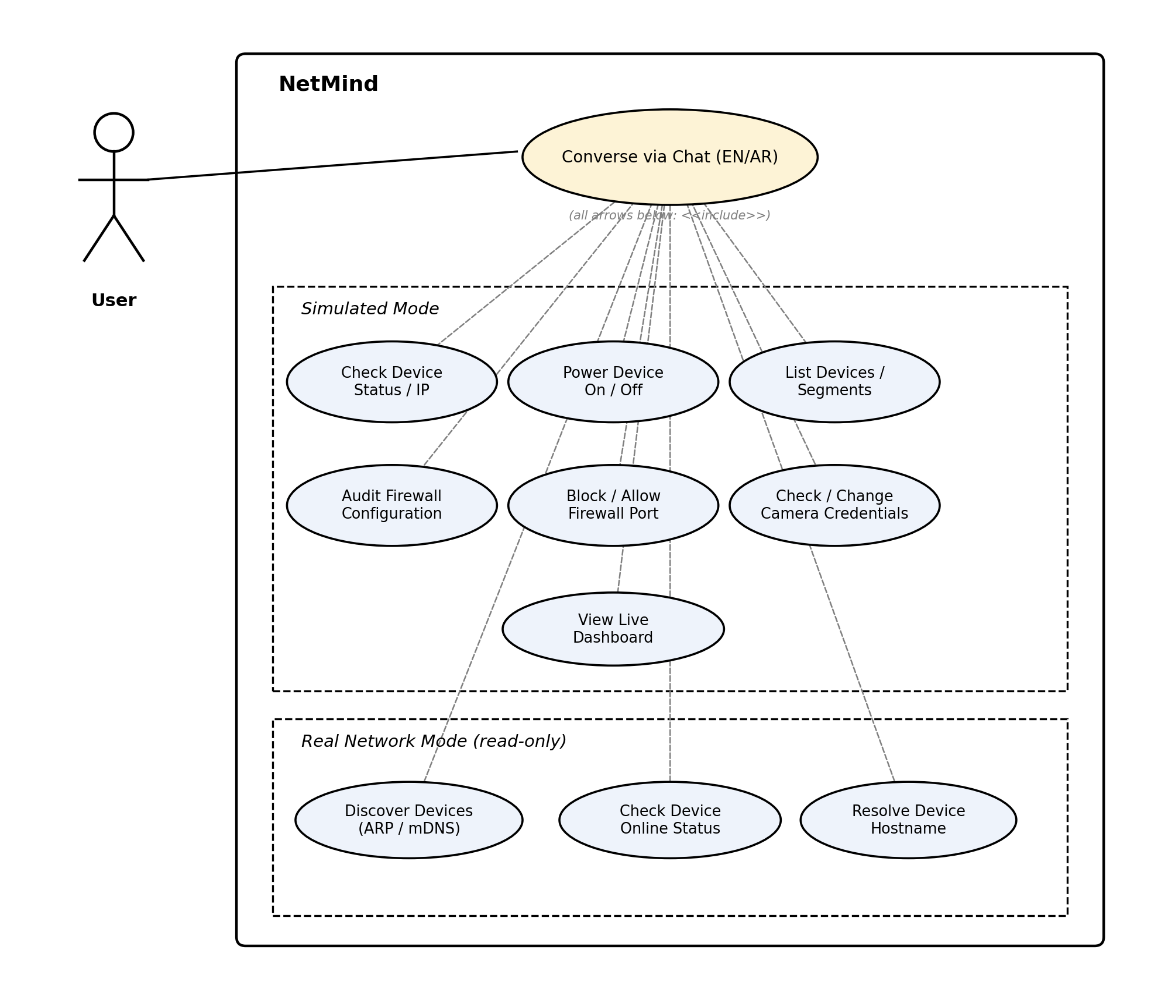
\includegraphics[width=0.78\textwidth]{use-case.png}
\caption{NetMind use case diagram}
\label{fig:usecase}
\end{figure}

\section{System Requirements}

\subsection{Clients, Customer and Users}

NetMind has no external paying customer; it is a Final Year Project built for
academic evaluation, so its requirements are shaped by three groups of
stakeholders. The primary users are the project team members themselves, who
use NetMind daily as network administrators-in-training against the
simulated lab network described in Chapter~5. The direct evaluators are the
project supervisor, Dr.\ Khalil Chebil, and the examining committee, who
assess the system against the functional and non-functional requirements set
out below. Beyond the project itself, NetMind is designed to be usable by any
operator of a small or medium branch network who would rather describe what
they want in natural language than memorise vendor-specific command-line
syntax; such an operator is assumed to have basic networking literacy, such
as knowing what a firewall port or a device IP address is, but not
necessarily fluency in any single configuration language, which is why the
system accepts both Arabic and English.

\subsection{Functional and Data Requirements}

The functional requirements gathered for NetMind are listed in
Table~\ref{tab:fr}.

NetMind's data lives in a small number of well-defined places rather than in
one large database. \code{registry.json}, generated by
\code{build\_registry.py}, is the static-plus-live mapping of each device's
id, owner, type, branch, segment, container name, management IP, and
simulated network IP; it is the single source every tool call resolves a
device name against. Conversation history and the audit log are stored in a
SQLite database (\code{logs/netmind.db}), so a chat session and the record of
every tool call survive a server restart; sessions are still bounded, with a
two-hour idle timeout, a cap of 200 sessions, and at most the system prompt
plus the 40 most recent messages per session. The alert history is kept in
\code{logs/alerts.json}. Device state itself, such as power status, firewall
rules, and camera stream status and credentials, is deliberately not
duplicated anywhere in NetMind: it is read live from Docker and from each
container, with only very short caches, so NetMind's picture cannot drift
from the lab. This removes an entire class of cache-invalidation bugs at the
cost of needing a reachable Docker daemon and live containers for every
query, which is acceptable for a lab environment and is discussed in
Chapter~6.

{\small
\begin{xltabular}{\textwidth}{|p{1.1cm}|Y|}
\hline
\head \textbf{ID} & \textbf{Functional Requirement} \\ \hline
\endhead
FR1 & The system shall allow a user to query the power status and IP address of any registered device by name or owner, tolerating small spelling mistakes in device names. \\ \hline
FR2 & The system shall allow a user to power a device on or off, shall report when the device is already in the requested state rather than performing a redundant action, and shall re-attach a powered-on device to its switch so that it is reachable again. \\ \hline
FR3 & The system shall allow a user to list every registered device, or every device on a specified network segment, validating segment names against the real topology. \\ \hline
FR4 & The system shall allow a user to list a firewall's configured rules, report which ports are open, and audit the firewall for common misconfigurations such as an administrative port left open to any source. Audits and rule listings shall cover both the INPUT chain (traffic to the firewall itself) and the FORWARD chain (traffic passing through it). \\ \hline
FR5 & The system shall allow a user to block or allow a specific port on a firewall. A block or allow shall take effect on both chains, so that it also stops or permits traffic between branches, and the change persists across a normal power cycle. \\ \hline
FR6 & The system shall allow a user to check whether a camera's video stream is reachable, start or stop that stream, and check or change the camera's credentials. \\ \hline
FR7 & In real-network mode, the system shall discover devices on the local network by combining ARP scanning, a ping sweep, IPv6 neighbour discovery and mDNS, and report each device once with its IPv4 address, IPv6 addresses, MAC address, hostname where available, online status and the methods that found it, without altering the state of any discovered device. \\ \hline
FR8 & The system shall accept user requests in either Arabic or English and reply in the same language as the request. \\ \hline
FR9 & The system shall refuse requests that are unrelated to network operations, and shall decline requests that reference a device outside the registry rather than guessing. \\ \hline
FR10 & The web dashboard shall display live device counts, status and open alerts obtained from the same backend state the chat assistant uses, polled at a regular interval, together with a permanent alert history (including when a device comes back online and how long it was down), an activity log of requested and confirmed actions, and a security and reliability report. \\ \hline
FR11 & The system shall not execute a destructive action (power off, block port, allow port, change camera credentials) on the language model's request alone. It shall create a pending action that only the user can confirm or cancel from the interface. \\ \hline
FR12 & Actions on protected devices (the core router and every firewall) shall require an additional explicit acknowledgement. \\ \hline
FR13 & Every tool call, and every confirmed, cancelled or expired destructive action, shall be recorded in an audit log with a timestamp, target, outcome and source. Passwords shall never be written to the log. \\ \hline
FR14 & The system shall allow a user to test whether one lab device can reach another over the simulated data network. \\ \hline
FR15 & The system shall be able to send alert and recovery notifications outside the browser (Telegram), including device, severity and timestamp. \\ \hline
\caption{Functional and data requirements}\label{tab:fr}\\
\end{xltabular}}

\subsection{Non-functional Requirements}

Beyond what NetMind must do, the following qualities were treated as
requirements in their own right, since a network tool that is slow, unsafe,
or hard to set up would not be used regardless of its feature list.

\subsubsection{Usability Requirement}

{\small
\begin{xltabular}{\textwidth}{|p{1.3cm}|Y|}
\hline
\head \textbf{ID} & \textbf{Non-functional Requirement} \\ \hline
\endhead
NFR1 & The system shall provide a single application combining chat and dashboard, requiring no separate manual or training to perform a basic device, firewall, or camera query. \\ \hline
NFR2 & The system shall accept and reply in either Arabic or English, matching the language of the user's request, and shall render structured results such as device or rule lists as formatted tables rather than raw text. \\ \hline
NFR3 & The system shall visually distinguish Simulated Mode from Real Network Mode at all times through an unambiguous, always-visible control. \\ \hline
\caption{Usability requirements}\label{tab:nfr-usability}\\
\end{xltabular}}

\subsubsection{Security Requirement}

{\small
\begin{xltabular}{\textwidth}{|p{1.3cm}|Y|}
\hline
\head \textbf{ID} & \textbf{Non-functional Requirement} \\ \hline
\endhead
NFR4 & Real Network Mode shall be strictly read-only: the real-network backend shall have no capability able to alter the state of any discovered device, enforced in code rather than by the prompt. \\ \hline
NFR5 & Every destructive action available in Simulated Mode, such as powering off a device, blocking or allowing a port, or changing a camera's credentials, shall be confined to the Containerlab lab environment. \\ \hline
NFR6 & The system shall require explicit user confirmation before executing a destructive action, with an additional acknowledgement for protected devices. \textbf{Implemented in Project 1} (Section~\ref{sec:guard}). \\ \hline
NFR12 & (Planned, Project 2) The system shall authenticate users, with roles, before granting access to the web interface. Not yet implemented; stated here as a known, scoped limitation rather than left unaddressed. \\ \hline
NFR13 & The server shall run as a normal user. The only privileges it needs (a raw socket for ARP scanning, and re-attaching a lab device to its bridge) shall be granted narrowly rather than by running the whole server as root. \\ \hline
\caption{Security requirements}\label{tab:nfr-security}\\
\end{xltabular}}

\subsubsection{Performance Requirement}

{\small
\begin{xltabular}{\textwidth}{|p{1.3cm}|Y|}
\hline
\head \textbf{ID} & \textbf{Non-functional Requirement} \\ \hline
\endhead
NFR7 & The agent loop shall cap tool-calling rounds at five per user request, so that no request can loop indefinitely. \\ \hline
NFR8 & The system shall use an LLM inference provider optimised for low response latency, since multi-step tool-calling compounds per-call latency directly into the user's perceived response time. \\ \hline
NFR9 & A real-network scan shall run its discovery methods in parallel, hold the mDNS browse window open for at least six seconds, and reuse a result for 20 seconds, so that repeated questions are answered instantly. \\ \hline
\caption{Performance requirements}\label{tab:nfr-performance}\\
\end{xltabular}}

\subsubsection{Portability Requirement}

{\small
\begin{xltabular}{\textwidth}{|p{1.3cm}|Y|}
\hline
\head \textbf{ID} & \textbf{Non-functional Requirement} \\ \hline
\endhead
NFR10 & The backend shall run on any Linux Docker host with Containerlab installed, including Windows via WSL2 with a native docker-ce installation, and the lab shall be deployable with one command. \\ \hline
NFR11 & The frontend shall require no installation beyond a standard web browser on the machine running NetMind. \\ \hline
\caption{Portability requirements}\label{tab:nfr-portability}\\
\end{xltabular}}

\subsubsection{Reliability Requirement}

{\small
\begin{xltabular}{\textwidth}{|p{1.3cm}|Y|}
\hline
\head \textbf{ID} & \textbf{Non-functional Requirement} \\ \hline
\endhead
NFR14 & Chat sessions, the audit log and the alert history shall survive a server restart. A storage failure shall never break a request. \\ \hline
NFR15 & Every change shall pass automated linting and unit tests, which shall run without Docker, a lab or an API key, before it is merged. \\ \hline
\caption{Reliability requirements}\label{tab:nfr-reliability}\\
\end{xltabular}}

% ============================================================
\chapter{Design Considerations}
% ============================================================

\section{Design Constraints}

Beyond the functional and non-functional requirements set out in Chapter~3,
three further constraints shaped how NetMind was designed: the hardware and
software environment the team actually had available, the characteristics of
the people the system is meant to serve, and the single academic term within
which a working system had to be built and demonstrated.

\subsection{Hardware and Software Environment}

NetMind had to run comfortably on each team member's own laptop rather than
on dedicated lab or cloud hardware, which ruled out heavier,
virtual-machine-based network emulators in favour of a lightweight,
container-based one. The simulated network alone comprises a core router,
three branch firewalls, three switch/hub segments, eight hosts, and three
cameras (eighteen nodes in total: fifteen containers and three bridge
segments), so the chosen tooling had to start, stop, and be queried quickly
without exhausting a single machine's resources. Because Docker Desktop's
bundled engine does not reliably expose the Linux network-namespace and
bridge access that Containerlab needs to wire virtual links between
containers, the team standardised on a native docker-ce engine running inside
a WSL2 Ubuntu distribution on each member's Windows machine, with
Containerlab itself used only once per deployment to build the topology from
a declarative YAML file. Figure~\ref{fig:environment} shows how the pieces of
this environment fit together, from the browser-based application down to
the simulated network itself and out to the external language-model
provider. Table~\ref{tab:environment} summarises the specific components of
this environment and the role each one plays.

\begin{figure}[H]
\centering
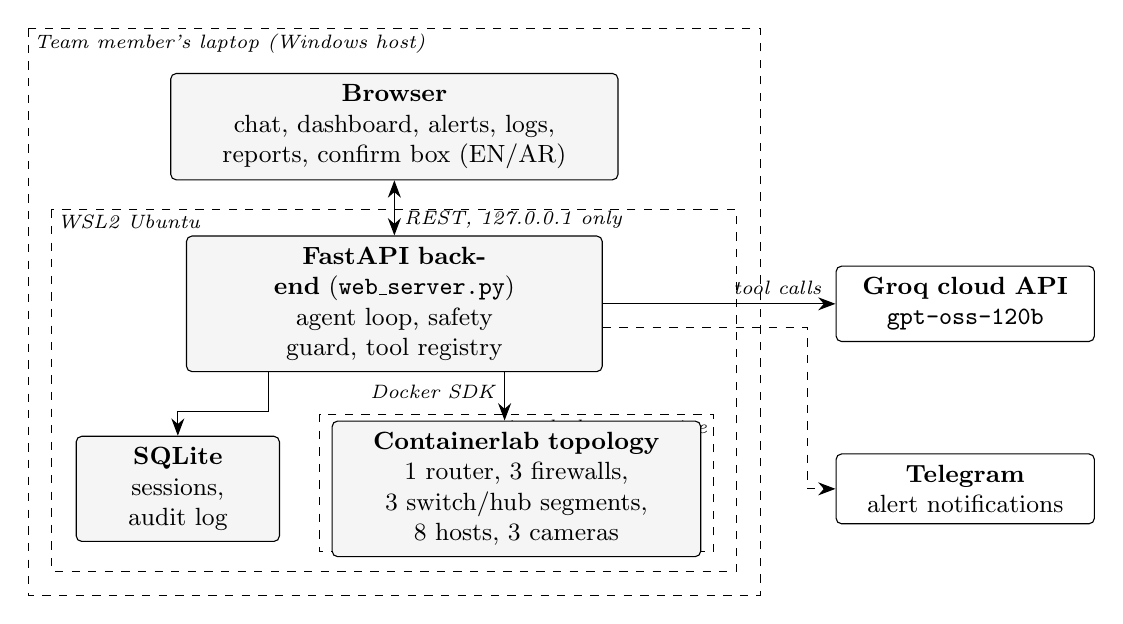
\begin{tikzpicture}[
  font=\small,
  box/.style={draw,rounded corners=2pt,fill=boxgray,align=center,inner sep=4pt},
  cloud/.style={box,fill=white},
  zl/.style={font=\scriptsize\itshape,anchor=north west,inner sep=2pt},
  note/.style={font=\scriptsize\itshape},
  >={Stealth[length=2.2mm]}]
  % zones (drawn first, explicit coordinates)
  \draw[dashed] (-0.3,0.3) rectangle (9.0,-6.9);
  \node[zl] at (-0.3,0.3) {Team member's laptop (Windows host)};
  \draw[dashed] (0.0,-2.0) rectangle (8.7,-6.6);
  \node[zl] at (0.0,-2.0) {WSL2 Ubuntu};
  \draw[dashed] (3.4,-4.6) rectangle (8.4,-6.35);
  \node[zl,anchor=north east] at (8.4,-4.6) {native docker-ce engine};
  % boxes
  \node[box,text width=5.4cm] (browser) at (4.35,-0.95)
    {\textbf{Browser}\\chat, dashboard, alerts, logs,\\reports, confirm box (EN/AR)};
  \node[box,text width=5.0cm] (api) at (4.35,-3.2)
    {\textbf{FastAPI backend} (\code{web\_server.py})\\agent loop, safety guard, tool registry};
  \node[box,text width=2.3cm] (db) at (1.6,-5.55) {\textbf{SQLite}\\sessions,\\audit log};
  \node[box,text width=4.4cm] (lab) at (5.9,-5.55)
    {\textbf{Containerlab topology}\\1 router, 3 firewalls,\\3 switch/hub segments,\\8 hosts, 3 cameras};
  \node[cloud,text width=3.0cm] (groq) at (11.6,-3.2) {\textbf{Groq cloud API}\\\code{gpt-oss-120b}};
  \node[cloud,text width=3.0cm] (tg) at (11.6,-5.55) {\textbf{Telegram}\\alert notifications};
  % arrows
  \draw[<->] (browser) -- node[right,note,pos=0.72]{REST, 127.0.0.1 only} (api);
  \draw[->] (api) -- node[above,note,pos=0.75]{tool calls} (groq);
  \draw[->,dashed] ([yshift=-3mm]api.east) -| (9.6,-5.55) -- (tg.west);
  \draw[->] ([xshift=-1.6cm]api.south) |- ++(0,-0.5) -| (db.north);
  \draw[->] ([xshift=1.4cm]api.south) -- node[left,note,pos=0.4]{Docker SDK} ([xshift=1.4cm]api.south |- lab.north);
\end{tikzpicture}
\caption{NetMind development and deployment environment}
\label{fig:environment}
\end{figure}

{\small
\begin{xltabular}{\textwidth}{|L{3.4cm}|Y|}
\hline
\head \textbf{Component} & \textbf{Role} \\ \hline
\endhead
Host OS & Windows 10/11 laptop belonging to each team member, running a WSL2 Ubuntu distribution \\ \hline
Container runtime & Native docker-ce engine inside WSL2 (not Docker Desktop's own engine) \\ \hline
Network emulation & Containerlab, used once per deployment to build the topology from a YAML file \\ \hline
Router node & FRRouting (\code{frrouting/frr}) image acting as the core router \\ \hline
Firewall nodes & Custom Alpine-based image running live iptables rules \\ \hline
Camera nodes & Custom Alpine-based image running a small Python HTTP service \\ \hline
Backend & Python 3 / FastAPI, communicating with Docker through the Docker SDK \\ \hline
Storage & SQLite (Python standard library) for chat sessions and the audit log; a JSON file for the alert history \\ \hline
Frontend & Vanilla JavaScript single-page application with chat, live dashboard, devices, alerts, logs and reports views, an in-page confirmation box, English/Arabic and light/dark themes, no build step \\ \hline
Language model & Groq API, \code{openai/gpt-oss-120b}, via an OpenAI-compatible tool-calling interface behind a provider interface \\ \hline
Notifications & Telegram Bot API (optional) for alerts outside the browser \\ \hline
Version control & Git, hosted on GitHub, with one issue per task and all changes merged by pull request \\ \hline
Continuous integration & GitHub Actions workflow running ruff and pytest, with a minimum test coverage, on every pull request \\ \hline
Lab automation & Makefile (\code{make up}, \code{make down}, \code{make run}, \code{make test}, \code{make lint}, \code{make setup-perms}) with idempotent bridge creation \\ \hline
\caption{Development and deployment environment}\label{tab:environment}\\
\end{xltabular}}

\subsection{End User Characteristics}

As set out in Chapter~3, NetMind is designed for an operator of a small or
medium branch network who may not be a dedicated network engineer: someone
comfortable with basic networking concepts such as an IP address or a
firewall port, but not necessarily fluent in any single vendor's command-line
syntax. Because the development team and the project's academic context are
Arabic-and-English bilingual, the same assumption was extended to language: a
user should be able to work entirely in whichever of the two languages they
are more comfortable in, without the system defaulting to one over the other.
Table~\ref{tab:users} summarises the characteristics assumed of this end user
and the design decision each one led to.

{\small
\begin{xltabular}{\textwidth}{|Y|Y|}
\hline
\head \textbf{Characteristic} & \textbf{Design Implication} \\ \hline
\endhead
Not a dedicated network engineer & Natural-language chat interface rather than a command-line or vendor-specific console (NFR1) \\ \hline
Comfortable in Arabic or English, not necessarily both equally & Bilingual input and output, matching the language of each request (NFR2) \\ \hline
Accesses the system from a standard laptop browser & No client installation; browser-only frontend (NFR13) \\ \hline
Expects a quick answer, not a slow diagnostic tool & Low-latency LLM provider and a bounded tool-calling loop (NFR9, NFR10) \\ \hline
May need to tell Simulated and Real Network mode apart at a glance & An always-visible control distinguishing the two modes (NFR3) \\ \hline
Responsible for device security, not just connectivity & Firewall auditing and camera credential checks exposed as first-class capabilities (FR4, FR6) \\ \hline
Is not always looking at the screen & Alerts kept as a history and sent to Telegram (FR10, FR15) \\ \hline
\caption{End-user characteristics and their design implications}\label{tab:users}\\
\end{xltabular}}

\section{Architectural Strategies}

\subsection{Development Method}

NetMind was built using an iterative, prototype-first method rather than a
single upfront design, an approach the supervisor, Dr.\ Khalil Chebil,
actively encouraged given the project's one-term timeline and its dependence
on infrastructure (the simulated network) that could only really be validated
once it existed. Each capability was built as a self-contained increment:
device status and power control first, then firewall auditing, then camera
security, and finally real-network discovery. Each increment was deployed
against the live Containerlab lab and reviewed with the supervisor before the
next one began, rather than being designed in isolation from working
infrastructure. Figure~\ref{fig:method} illustrates this loop.

\begin{figure}[H]
\centering
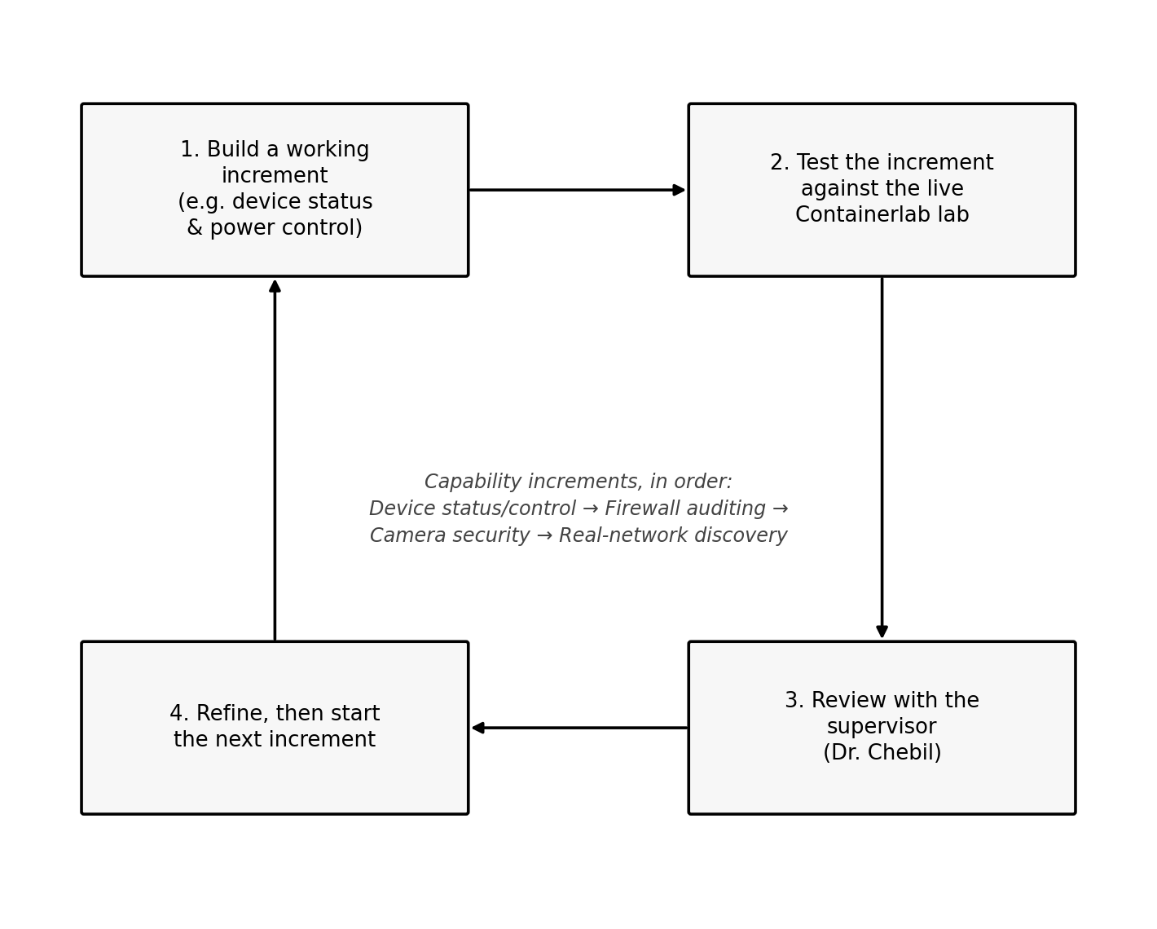
\includegraphics[width=0.72\textwidth]{dev-method.png}
\caption{Iterative, supervisor-reviewed development method}
\label{fig:method}
\end{figure}

This incremental approach meant that a demonstrable, working system existed
from early in the project, and that any gaps a given increment left behind
were identified against a real, running lab rather than assumed away on
paper. At the end of September the supervisor reviewed the whole system and
prepared an assessment and a seven-month improvement plan (October 2026 to
April 2027) organised as monthly milestones. From October onwards the team
therefore worked from that plan: every task became a GitHub issue, every
change was made on its own branch and merged through a pull request that
needed the continuous-integration checks to pass, and the work was split
across three tracks (core backend, AI agent, and frontend and real network)
so that each member has individually assessable contributions. The first two
milestones, stabilisation (October) and the architecture refactor
(November), are complete.

\subsection{Future Enhancements and Plans}

The current system intentionally leaves work for Project 2. The supervisor's
plan sets out the remaining milestones, and the team has added two items of
its own that build directly on the existing tool registry and agent loop.
Table~\ref{tab:p2plan} outlines the main areas; Section~6.3 lists them in
more detail.

{\small
\begin{xltabular}{\textwidth}{|L{3.2cm}|Y|}
\hline
\head \textbf{Area} & \textbf{Planned Enhancement} \\ \hline
\endhead
Observability & A background collector with a per-device state machine, so alerts are raised even when nobody has the dashboard open; diagnostic and alert-history tools for the agent \\ \hline
Diagnosis & Reversible fault-injection scenarios and root-cause-analysis playbooks that diagnose a fault with evidence \\ \hline
Safe change & Proactive fix suggestions, firewall snapshots with diff and rollback, and authentication with roles (NFR7) \\ \hline
Evaluation & A benchmark of 100+ English and Arabic prompts, a comparison of LLM providers and models, load testing, and a usability study \\ \hline
Integration & An MCP server exposing NetMind's tools to other AI assistants, and a hardened agent harness \\ \hline
\caption{Planned enhancements for Project 2}\label{tab:p2plan}\\
\end{xltabular}}

% ============================================================
\chapter{System Design}
% ============================================================

\section{System Architecture and Program Flow}

NetMind's architecture separates four concerns: deploying the network,
resolving device names to real network identities, deciding what action to
take, and checking that the action is allowed before it runs.

\textbf{Deployment.} Containerlab is used only once per deployment:
\code{generate\_topology.py} builds a topology YAML file from a Python
description of the branches and devices (\code{branches.py}, the single
source of truth for the layout and IP plan), and \code{containerlab deploy}
creates the actual Docker containers and virtual links. \code{make up} runs
the whole sequence, including the idempotent creation of the Linux bridges
that act as switches and hubs. After this point Containerlab is no longer
involved; every device is simply an ordinary Docker container.

\textbf{The device registry.} Because container names and IP addresses are
only known once Containerlab has deployed them, \code{build\_registry.py}
runs \code{containerlab inspect}, cross-references the live state against the
static branch design, and writes a single \code{registry.json} mapping each
device's name and owner to its real container name and IP addresses. This
registry, not Containerlab, is what the rest of the system queries at runtime.

\textbf{Services and backends.} All lab logic lives in three typed services
(\code{DeviceService}, \code{FirewallService} and \code{CameraService} in
\code{services.py}) which use the Docker SDK to start and stop containers
and to execute commands inside them, such as running iptables inside a
firewall or requesting a camera's stream. The outside world (the Docker
client, the registry loader) is passed into each service, so every service
can be tested with plain fakes. The services sit behind a
\code{NetworkBackend} interface with two implementations: a
\code{ContainerlabBackend} for the simulated lab and a
\code{RealLanBackend} for the physical network. Each backend declares the
capabilities it has, and a tool whose capability the backend lacks is
refused in code.

\textbf{The language model layer.} Every tool the model can use is one
registered Python function (\code{tool\_catalog.py}); its schema is built
from the function's name, type hints and docstring, and its decorator records
the capability it needs and its risk level. The web server sends the user's
message and the schemas of the active mode's tools to the model through a
provider interface. The model decides whether to reply directly or to call
one or more tools; each call passes through the safety guard
(Section~\ref{sec:guard}), the result is fed back to the model, and this
repeats for up to five rounds until a final reply is produced. The language
model therefore never touches Docker or Containerlab directly; it only sees
named tools and their results, which is also what lets the same model operate
the separate real-network mode simply by swapping the backend.
Figure~\ref{fig:programflow} shows the deploy-time path and the runtime
loop, and Figure~\ref{fig:layers} shows the layers a tool call passes
through.

\begin{figure}[H]
\centering
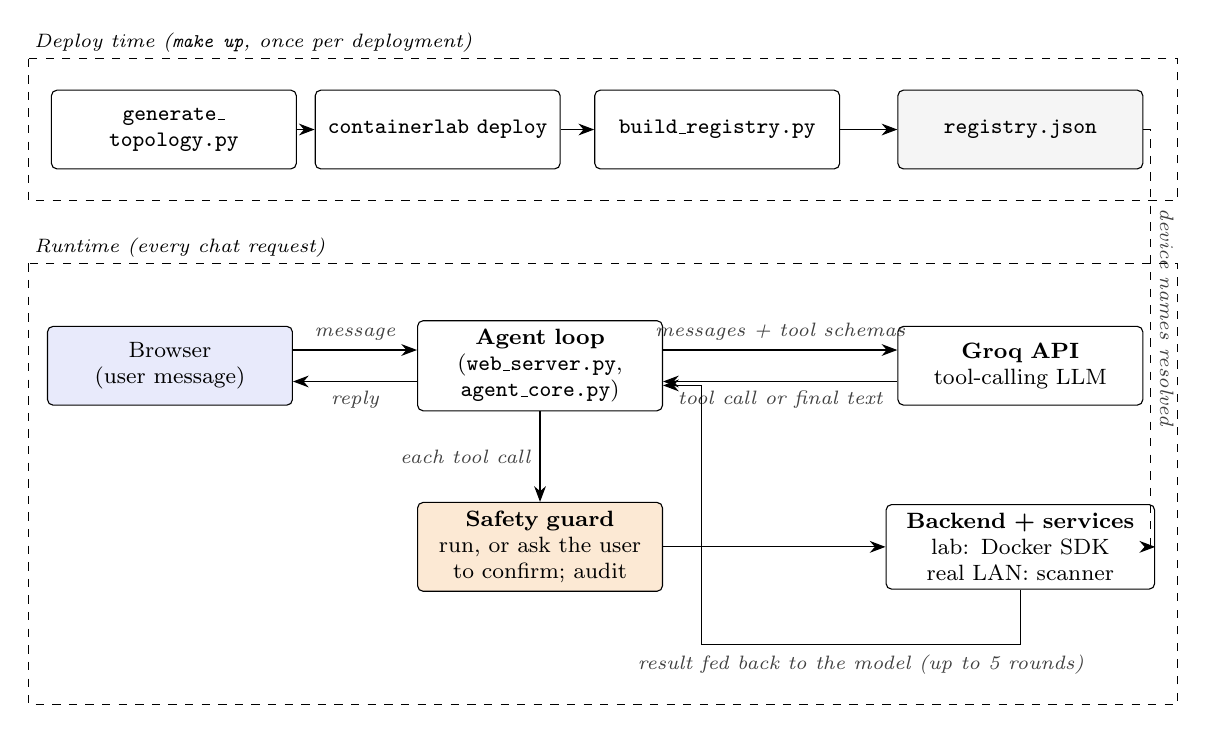
\begin{tikzpicture}[
  font=\footnotesize,
  box/.style={draw,rounded corners=2pt,fill=white,align=center,minimum height=1.0cm,inner sep=3pt,text width=2.9cm},
  zl/.style={font=\scriptsize\itshape,anchor=south west,inner sep=2pt},
  note/.style={font=\scriptsize\itshape,text=black!75},
  >={Stealth[length=2mm]}]
  % deploy time
  \draw[dashed] (-0.2,0.9) rectangle (14.4,-0.9);
  \node[zl] at (-0.2,0.9) {Deploy time (\code{make up}, once per deployment)};
  \node[box] (gen) at (1.65,0) {\code{generate\_topology.py}};
  \node[box] (dep) at (5.0,0) {\code{containerlab deploy}};
  \node[box] (reg) at (8.55,0) {\code{build\_registry.py}};
  \node[box,fill=boxgray] (json) at (12.4,0) {\textbf{\code{registry.json}}};
  \draw[->] (gen) -- (dep); \draw[->] (dep) -- (reg); \draw[->] (reg) -- (json);
  % runtime
  \draw[dashed] (-0.2,-1.7) rectangle (14.4,-7.3);
  \node[zl] at (-0.2,-1.7) {Runtime (every chat request)};
  \node[box,fill=userblue] (chat) at (1.6,-3.0) {Browser\\(user message)};
  \node[box] (ws) at (6.3,-3.0) {\textbf{Agent loop}\\(\code{web\_server.py},\\\code{agent\_core.py})};
  \node[box] (llm) at (12.4,-3.0) {\textbf{Groq API}\\tool-calling LLM};
  \node[box,fill=guardorange] (guard) at (6.3,-5.3) {\textbf{Safety guard}\\run, or ask the user\\to confirm; audit};
  \node[box,text width=3.2cm] (be) at (12.4,-5.3) {\textbf{Backend + services}\\lab: Docker SDK\\real LAN: scanner};
  \draw[->] ([yshift=2mm]chat.east) -- node[above,note]{message} ([yshift=2mm]ws.west);
  \draw[->] ([yshift=-2mm]ws.west) -- node[below,note]{reply} ([yshift=-2mm]chat.east);
  \draw[->] ([yshift=2mm]ws.east) -- node[above,note]{messages + tool schemas} ([yshift=2mm]llm.west);
  \draw[->] ([yshift=-2mm]llm.west) -- node[below,note]{tool call or final text} ([yshift=-2mm]ws.east);
  \draw[->] (ws) -- node[left,note]{each tool call} (guard);
  \draw[->] (guard) -- (be);
  \draw[->] (be.south) -- ++(0,-0.7) -| node[pos=0.25,below,note]{result fed back to the model (up to 5 rounds)} (8.35,-3.25) -- (8.35,-3.25 -| ws.east);
  \draw[->,dashed] (json.east) -- (14.05,0) -- node[pos=0.45,sloped,above,note]{device names resolved} (14.05,-5.3) -- (be.east);
\end{tikzpicture}
\caption{NetMind program flow, showing the deploy-time path and the runtime tool-calling loop}
\label{fig:programflow}
\end{figure}

\begin{figure}[H]
\centering
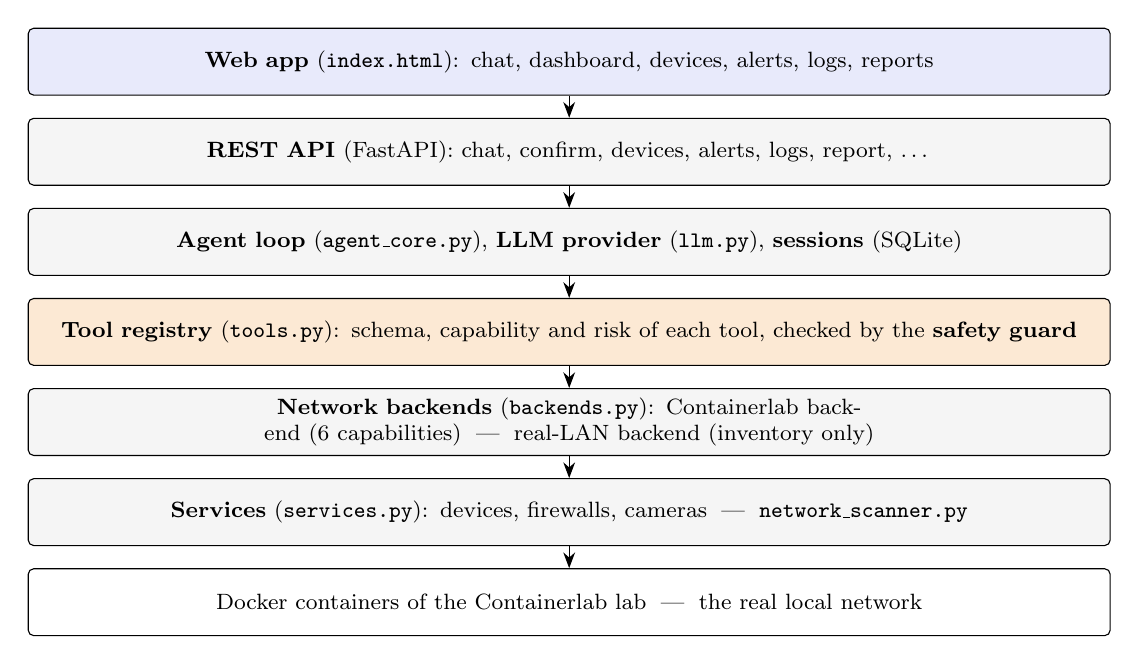
\begin{tikzpicture}[
  font=\footnotesize,
  layer/.style={draw,rounded corners=2pt,text width=13.6cm,minimum height=0.85cm,align=center,fill=boxgray,inner sep=2pt},
  >={Stealth[length=2mm]}, node distance=0.28cm]
  \node[layer,fill=userblue] (ui) {\textbf{Web app} (\code{index.html}): chat, dashboard, devices, alerts, logs, reports};
  \node[layer,below=of ui] (api) {\textbf{REST API} (FastAPI): chat, confirm, devices, alerts, logs, report, \dots};
  \node[layer,below=of api] (agent) {\textbf{Agent loop} (\code{agent\_core.py}), \textbf{LLM provider} (\code{llm.py}), \textbf{sessions} (SQLite)};
  \node[layer,below=of agent,fill=guardorange] (reg) {\textbf{Tool registry} (\code{tools.py}): schema, capability and risk of each tool, checked by the \textbf{safety guard}};
  \node[layer,below=of reg] (be) {\textbf{Network backends} (\code{backends.py}): Containerlab backend (6 capabilities) \;|\; real-LAN backend (inventory only)};
  \node[layer,below=of be] (svc) {\textbf{Services} (\code{services.py}): devices, firewalls, cameras \;|\; \code{network\_scanner.py}};
  \node[layer,below=of svc,fill=white] (world) {Docker containers of the Containerlab lab \;|\; the real local network};
  \foreach \a/\b in {ui/api,api/agent,agent/reg,reg/be,be/svc,svc/world} \draw[->] (\a) -- (\b);
\end{tikzpicture}
\caption{Layers a request passes through after the November refactor}
\label{fig:layers}
\end{figure}

\section{Detailed Design}

\subsection{Detailed Component Description}

\para{Simulated Network Device Control Module}

NetMind's simulated mode operates against a virtual network built with
Containerlab: a core router, three branch firewalls, three switch or hub
segments, eight hosts, and three IP cameras, connected with real IP
addressing and routing between branches. This module exposes five groups of
capabilities to the language model, summarised in Table~\ref{tab:simcaps}.

\textbf{Device status and control.} Reporting whether a host, firewall,
camera, or router is online or offline, retrieving its IP address, and
powering it on or off. Device names are matched exactly by id or owner first
and then, for small spelling mistakes, by a careful fuzzy match that only
accepts one clearly best candidate. Power operations are idempotent, so a
request to power on an already-running device is reported as no change
rather than a false action. Because stopping a container deletes the virtual
link Containerlab created, powering a host or camera back on re-attaches it
to its switch and replays its addressing and routes, then checks that it can
reach its gateway.

\textbf{Network visibility and connectivity.} Listing every device with its
owner, type, and status, listing the devices on a specific switch or hub
segment, validating the segment name against the real topology rather than
silently returning an empty result, and pinging one device from another over
the lab's data network (not the management network, which would hide a
broken link).

\textbf{Firewall auditing.} Each branch firewall runs a real Linux iptables
firewall rather than a placeholder. NetMind can list its configured rules,
report open ports, audit it for common misconfigurations such as an
administrative port left open to any source, and block or allow a port on
request; changes persist across a normal power cycle. Rules are applied to
both the INPUT chain and the FORWARD chain, because a rule on INPUT alone
only protects the firewall itself and does not stop traffic passing through
it between branches; an integration test confirms this with real traffic
(Section~\ref{sec:testing}). Rule changes are idempotent: NetMind checks
whether a rule already exists before inserting it, so repeating a request
never creates duplicates.

\textbf{Camera security.} Each camera runs a small real HTTP service, so
NetMind can check whether its stream is actually reachable independently of
the device's power state, start or stop the stream service, and check or
change the camera's default password.

{\small
\begin{xltabular}{\textwidth}{|L{3.6cm}|Y|}
\hline
\head \textbf{Capability Group} & \textbf{What It Provides} \\ \hline
\endhead
Device status and control & Online/offline status, IP address, and idempotent power on/off for any host, firewall, camera, or router, with automatic re-attachment after power-on \\ \hline
Network visibility & Listing every device, or every device on a specific switch/hub segment, validated against the real topology \\ \hline
Connectivity & Pinging one lab device from another over the data network \\ \hline
Firewall auditing & Listing configured iptables rules (INPUT and FORWARD chains), reporting open ports, auditing for misconfigurations, and blocking/allowing ports \\ \hline
Camera security & Checking stream reachability independently of power state, starting/stopping the stream, and checking/changing the default password \\ \hline
\caption{Simulated-mode capability groups (summary)}\label{tab:simcaps}\\
\end{xltabular}}

All of this runs over genuine IP addressing and routing between branches
rather than a flat management network, verified through packet round-trip
testing and Time-To-Live analysis to confirm that traffic between branches
actually traverses the intended switch, firewall, and router path.

\para{Real Network Discovery Module}

The real network discovery module is the component that gives NetMind
visibility of an actual physical network. It is written in Python and is
deliberately read-only: it observes the local network and reports what it
finds, but it never changes the state of any device. This is what separates
it from the device control module, which manages the Docker containers of the
simulated Containerlab network. Keeping the two apart means that every
operation which can change a device is confined to the simulated
environment, while the real network can only be observed, which removes any
risk of the language model accidentally altering a live network. The
boundary is enforced by the backend: \code{RealLanBackend} has only the
inventory capability, so the power, firewall and camera tools cannot run
against it whatever the model asks.

The module exposes three functions to the tool layer: listing the devices on
the network, checking whether a single device is online, and resolving a
hostname to an IP address. Each device is returned once, as a dictionary
containing its IPv4 address, its IPv6 addresses, its MAC address, its
hostname, its status, and \code{found\_by}, the list of discovery methods
that saw it. The dashboard shows \code{found\_by} for every device.

\textbf{Program flow.} The first version of the module ran ARP and fell back
to a ping sweep only when ARP could not run, so a scan reported the devices
found by one method only, even though each method finds devices the other
misses. In November the scan was redesigned so that all methods run at the
same time and their results are merged. Table~\ref{tab:scansteps} lists the
stages of a scan and Figure~\ref{fig:scanflow} shows the flow.

{\small
\begin{xltabular}{\textwidth}{|>{\centering\arraybackslash}p{0.8cm}|L{3.2cm}|Y|}
\hline
\head \textbf{Step} & \textbf{Stage} & \textbf{Description} \\ \hline
\endhead
1 & Subnet detection & The local subnet is derived from the machine's own IP address on its default route, so that no configuration is needed from the user. \\ \hline
2 & Parallel discovery & Four methods start together: a broadcast ARP request to every address in the subnet (IP and MAC of each device that answers); a ping sweep of the subnet with 64 parallel workers; an mDNS browse of six seconds that maps addresses to the names devices advertise; and a ping to the IPv6 all-nodes address so that IPv6 neighbours appear in the kernel's neighbour table. A method that cannot run, such as ARP without raw-socket permission, is reported as not run, and the others still complete. \\ \hline
3 & Merge & Devices are merged by IPv4 address. Each keeps the list of methods that found it. A device found only by ping takes its MAC address from the kernel's neighbour table. \\ \hline
4 & IPv6 matching & IPv6 addresses from the neighbour table are attached to the device with the same MAC address. \\ \hline
5 & Hostname resolution & For each device the hostname is taken from the mDNS table if present, and otherwise from a reverse DNS lookup, done in parallel. \\ \hline
6 & Output & The list is sorted by address and returned with the methods that ran; it is cached for 20 seconds. \\ \hline
\caption{Real-network discovery module program flow steps}\label{tab:scansteps}\\
\end{xltabular}}

\begin{figure}[H]
\centering
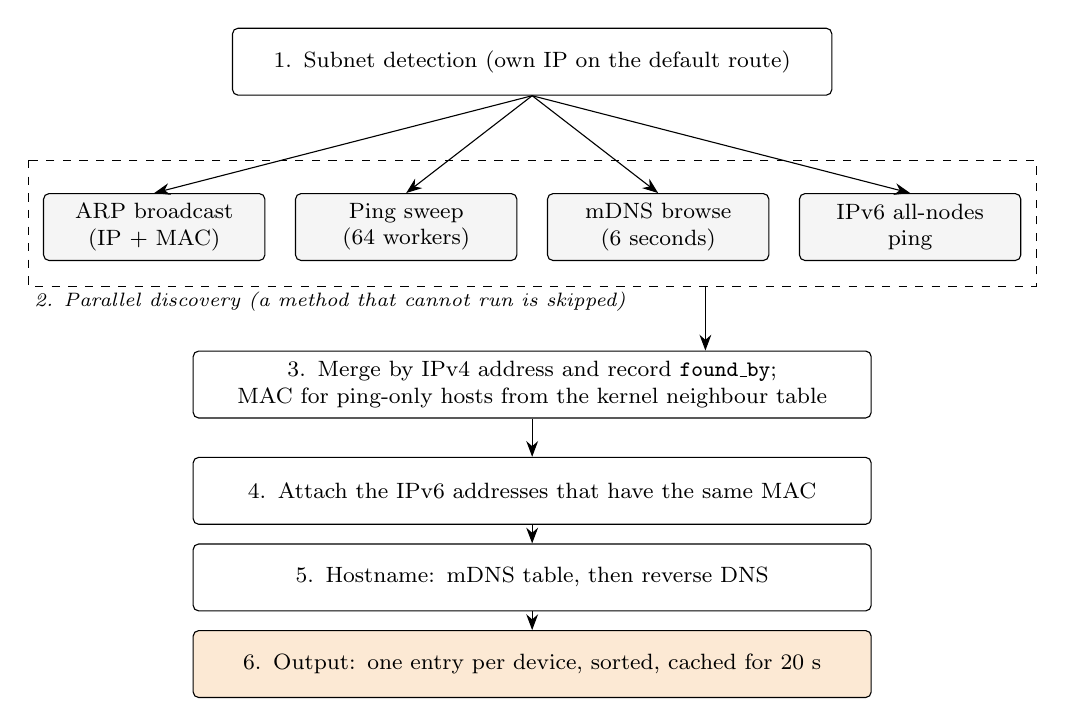
\begin{tikzpicture}[
  font=\footnotesize,
  box/.style={draw,rounded corners=2pt,fill=white,align=center,minimum height=0.85cm,inner sep=3pt},
  par/.style={box,fill=boxgray,text width=2.6cm},
  >={Stealth[length=2mm]}]
  \node[box,text width=7.4cm] (sub) at (6.3,0) {1. Subnet detection (own IP on the default route)};
  \node[par] (arp)  at (1.5,-2.1) {ARP broadcast\\(IP + MAC)};
  \node[par] (ping) at (4.7,-2.1) {Ping sweep\\(64 workers)};
  \node[par] (mdns) at (7.9,-2.1) {mDNS browse\\(6 seconds)};
  \node[par] (ndp)  at (11.1,-2.1) {IPv6 all-nodes\\ping};
  \draw[dashed] (-0.1,-1.25) rectangle (12.7,-2.85);
  \node[font=\scriptsize\itshape,anchor=north west,inner sep=2pt] at (-0.1,-2.85) {2. Parallel discovery (a method that cannot run is skipped)};
  \node[box,text width=8.4cm] (merge) at (6.3,-4.1) {3. Merge by IPv4 address and record \code{found\_by};\\MAC for ping-only hosts from the kernel neighbour table};
  \node[box,text width=8.4cm] (v6) at (6.3,-5.45) {4. Attach the IPv6 addresses that have the same MAC};
  \node[box,text width=8.4cm] (host) at (6.3,-6.55) {5. Hostname: mDNS table, then reverse DNS};
  \node[box,text width=8.4cm,fill=guardorange] (out) at (6.3,-7.65) {6. Output: one entry per device, sorted, cached for 20 s};
  \foreach \n in {arp,ping,mdns,ndp} \draw[->] (sub.south) -- (\n.north);
  \draw[->] (8.5,-2.85) -- (8.5,-3.45 |- merge.north);
  \draw[->] (merge) -- (v6); \draw[->] (v6) -- (host); \draw[->] (host) -- (out);
\end{tikzpicture}
\caption{Real-network discovery module program flow}
\label{fig:scanflow}
\end{figure}

\textbf{Design Decisions and Alternatives Considered.} This part explains why
each technique and library was chosen, and which alternatives were considered
and not selected (summary in Table~\ref{tab:decisions}).

{\small
\begin{xltabular}{\textwidth}{|L{3.2cm}|Y|}
\hline
\head \textbf{Decision} & \textbf{Chosen Approach (Alternatives Considered)} \\ \hline
\endhead
Subnet detection & UDP socket trick, standard library only, with \code{ip addr} as a fallback (netifaces/psutil: accurate but an extra dependency; gethostbyname: often returns 127.0.0.1) \\ \hline
Host discovery & ARP via Scapy and a ping sweep, run together and merged (Nmap: more capable but a heavier external binary; arp-scan: external dependency; OS ARP cache alone: misses undiscovered hosts; passive sniffing: slow) \\ \hline
IPv6 discovery & Ping the all-nodes multicast address, then read the kernel neighbour table (a full IPv6 sweep: impossible, a /64 has $2^{64}$ addresses) \\ \hline
Concurrency & ThreadPoolExecutor: one pool for the four methods, 64 workers for the ping sweep (multiprocessing: heavier for I/O-bound work; asyncio: would need a restructured codebase) \\ \hline
Hostname discovery & mDNS via zeroconf (NetBIOS: Windows-only; SSDP/UPnP: fewer device types; DHCP leases: needs router access; SNMP: needs credentials) \\ \hline
Reverse DNS & Python standard library, used as a secondary source \\ \hline
Status checking & A single ping (TCP connect or ARP probe identified as possible improvements) \\ \hline
Optional dependencies & Scapy and zeroconf imported in try/except, so the module degrades gracefully if either is missing \\ \hline
Privileges & A copy of the virtualenv's Python with only the raw-socket capability, so ARP works without running the server as root \\ \hline
\caption{Design decisions and alternatives considered (summary)}\label{tab:decisions}\\
\end{xltabular}}

\textbf{Subnet detection.} The active interface is found by opening a UDP
socket towards a public address and reading the local address the operating
system assigns to it. No packet is actually sent, and the method relies only
on the Python standard library. If there is no default route at all, the
module reads the interface configuration with \code{ip addr} instead.
Alternatives were the netifaces and psutil libraries, which are more accurate
on machines with several interfaces but add an external dependency, and
gethostbyname applied to the machine's own hostname, which frequently returns
the loopback address 127.0.0.1 and is therefore unreliable. The chosen method
assumes a /24 subnet, which is a known limitation.

\textbf{Host discovery with ARP, Scapy and a ping sweep.} ARP was chosen
because it works at the data link layer: a device cannot ignore an ARP
request and still take part in an Ethernet network, so ARP finds devices that
are configured to block ICMP ping, and it also returns the MAC address. Scapy
was chosen to send the requests because it is a pure Python library that
integrates directly with the rest of the code and gives full control over
packet construction without an external program. In practice, however, some
devices answer ping but miss the short ARP window, so the ping sweep is not
only a fallback: running both and merging the results finds more devices than
either method alone, and \code{found\_by} makes visible which method saw each
device. The alternatives were Nmap, used directly or through python-nmap,
which is far more capable but is a separate binary larger than this module
requires; the arp-scan command-line tool, which is fast but is again an
external dependency; the operating system's ARP cache, which only lists
devices that the machine has already communicated with; and passive sniffing
of network traffic, which needs no probes but can take a long time to reveal
quiet devices.

\textbf{IPv6.} An IPv6 subnet is far too large to sweep, so the module sends
one ping to the IPv6 all-nodes multicast address on the active interface. Every
IPv6 device on the link answers, which places it in the kernel's neighbour
table; the module then reads that table and attaches each IPv6 address to the
device with the same MAC address. A device often has several IPv6 addresses
(a link-local \code{fe80::} address and one or more global ones), and all are
listed.

\textbf{Concurrency.} Checking 254 addresses one after another would take
several minutes, since each unanswered ping waits up to one second. A
ThreadPoolExecutor with 64 workers runs the pings in parallel and reduces the
sweep to a few seconds, and a second small pool runs the four discovery
methods at the same time, so a full scan takes about as long as its slowest
method. Threads suit this task because it is bound by waiting on the network
rather than by computation. The alternatives were multiprocessing, whose
separate processes add memory and start-up cost for work that is only
waiting, and asyncio, which would be efficient but would require the
surrounding code to be restructured around asynchronous functions.

\textbf{Hostname discovery with mDNS.} Multicast DNS was chosen because small
and home networks often have no reverse DNS records, so a reverse lookup
alone returns no name for most devices. mDNS lets printers, AirPlay devices,
Chromecast devices, and shared workstations announce their names without any
credentials or access to the router, and the zeroconf library provides a pure
Python implementation. The browse runs on every scan rather than once at
server start, so that a device that joins the network later is still found.
The alternatives were NetBIOS name queries, which are mostly limited to
Windows hosts; SSDP and UPnP discovery, which cover fewer device types; DHCP
lease tables read from the router, which need administrative access to the
router; and SNMP queries, which need SNMP to be enabled and credentials to be
known. A limitation of mDNS is that a device which advertises no service, such
as an idle phone, appears without a hostname, although it is still listed by
IP and MAC address.

\textbf{Reverse DNS and status checking.} Reverse DNS through the standard
library is used as a secondary source, because it is already available in
Python at no cost and gives names on networks that do maintain DNS records.
The status of a single device is determined with one ping, which keeps it
consistent with the ping sweep and needs no extra dependency. A TCP
connection check or an ARP probe would be more reliable against devices that
block ICMP, and are identified as possible improvements.

\textbf{Optional dependencies and output format.} Scapy and zeroconf are
imported inside try and except blocks, and their availability is recorded in
flags. If either library is missing the module degrades gracefully instead of
failing to start, which makes it easier to run on different machines. Results
are returned as plain dictionaries, rather than custom classes, because they
map directly to JSON for the API.

\textbf{Limitations.} ARP scanning only works within the local broadcast
domain and needs the raw-socket capability. The ping command options used are
those of Linux and would have to be adapted for Windows and macOS. A device
that blocks ICMP may be reported as offline by the status check. The subnet is
assumed to be a /24. Under WSL2's default network mode the scanner sees the
virtual network between Windows and WSL rather than the physical LAN, so real
mode needs WSL's mirrored networking mode or a native Linux machine. Finally,
network scanning should only be carried out on networks owned by the user or
for which permission has been given.

\para{Live Monitoring Dashboard Module}

The live monitoring dashboard is the module that gives the operator a single,
continuously updated view of the network without having to ask the chat
interface a question first. It is implemented as part of a unified
single-page application that also hosts the chat interface, so both views
share one navigation shell, one theme, one language setting, and one REST
client rather than being two separate pages. Table~\ref{tab:dashcaps}
summarises its capability groups.

{\small
\begin{xltabular}{\textwidth}{|L{3.6cm}|Y|}
\hline
\head \textbf{Capability Group} & \textbf{What It Provides} \\ \hline
\endhead
Unified application shell & One entry point providing both the chat and dashboard views, with shared sidebar navigation, light/dark theme, Arabic/English language switching, and a single REST client used by both views \\ \hline
Mode-aware refresh & Polls \code{/api/devices} and \code{/api/alerts} (simulated) or \code{/api/real-devices} and \code{/api/real-alerts} (real network) on a fixed interval, discarding any response that no longer matches the currently selected mode to avoid a stale-data race \\ \hline
Network visibility & Renders device and connection state, live statistics (online/offline counts), a topology view, and an active-alerts panel from the same registry data used by the chat tools \\ \hline
Device inventory view & A dedicated devices page listing currently active devices, with best-effort device-type classification (laptop, phone, router, etc.) from MAC OUI prefixes and hostname heuristics, each shown with a type icon; in real mode it also shows how each device was found \\ \hline
Evidence chain & Each chat reply that triggers one or more backend tool calls is accompanied by a collapsible, step-by-step trace of which tool was called, with what arguments, and what it returned, so the operator can inspect the reasoning behind a diagnosis rather than trusting it blindly \\ \hline
\caption{Live monitoring dashboard capability groups (summary)}\label{tab:dashcaps}\\
\end{xltabular}}

\textbf{Design decisions.} The dashboard and chat interface were originally
built as two separate HTML pages and were later merged into one application
shell, each view kept in its own section and toggled client-side without a
page reload, so that navigation state, theme, language, and the active
network mode persist across both views instead of resetting. The refresh
logic is deliberately race-safe: each poll captures which mode it was
requested for, and a response is applied to the interface only if that mode
is still the one selected when the response arrives, which prevents
simulated-network data from briefly overwriting real-network data (or vice
versa) when the operator switches modes while a request is in flight.
Device-type classification in the inventory view is explicitly best-effort
only: modern phones that randomise their MAC address (iOS 14+/Android 10+)
cannot be reliably identified by OUI lookup, so the interface documents this
limitation rather than presenting the classification as certain.

\textbf{Limitation.} Like the rest of the frontend, the dashboard has no
authentication and assumes a single trusted operator, consistent with the
scoped-out security requirement (NFR12) already noted in Chapter~3.

% ------------------------------------------------------------
\subsection{Safety Guard: Confirmation, Protected Devices and Audit Log}
\label{sec:guard}

A language model that can call tools can also be wrong or be misled by a
request, so NetMind does not let the model carry out destructive actions
itself. Every tool is registered with one of three risk levels. \emph{Read}
tools (status, listings, audits, pings) run immediately. \emph{Action} tools,
which change state but are easy to undo (power on, start or stop a camera
stream), also run immediately and are audited. \emph{Destructive} tools
(power off, block port, allow port, and change camera credentials) never run
on the model's call. Because the risk level is part of the tool's
registration, the guard, the backends and the dashboard all read it from the
same table, and a new tool cannot be added without one.

When the model calls a destructive tool, the guard does not run the action.
It stores a pending action containing the tool, its target, and its
arguments, and returns a ``pending'' result to the model. The pending action
is shown to the user in the chat as a Confirm/Cancel box. The action runs only
when the user presses Confirm, which sends a request to a separate endpoint
(\code{POST /api/confirm}) that the model has no way to call. A pending action
that is not answered within five minutes expires.
Figure~\ref{fig:confirm} shows the sequence.

The core router and every firewall are classed as protected devices.
Confirming an action on a protected device requires the user to tick an
additional acknowledgement box, and the server rejects the request without
it.

Every outcome (executed, cancelled, expired, or rejected) is written to an
audit log, stored in the SQLite database and also appended to
\code{logs/audit.jsonl}. Each entry records the time, the tool, the target,
the outcome, and the result. Camera passwords are redacted before an entry is
written.

Language models sometimes answer an action request in text, for example
saying that a request is ``pending'', without calling any tool. In that case
the user would see no Confirm box and nothing would happen. To catch this,
the agent loop checks the reply against two patterns: a destructive request
that produced no tool call, and a reply that claims something is pending or
done. When either matches, the loop retries once with an explicit instruction
to call the tool. This retry is a safety net for usability and does not weaken
the guard, because no path from the model leads to execution.

\begin{figure}[H]
\centering
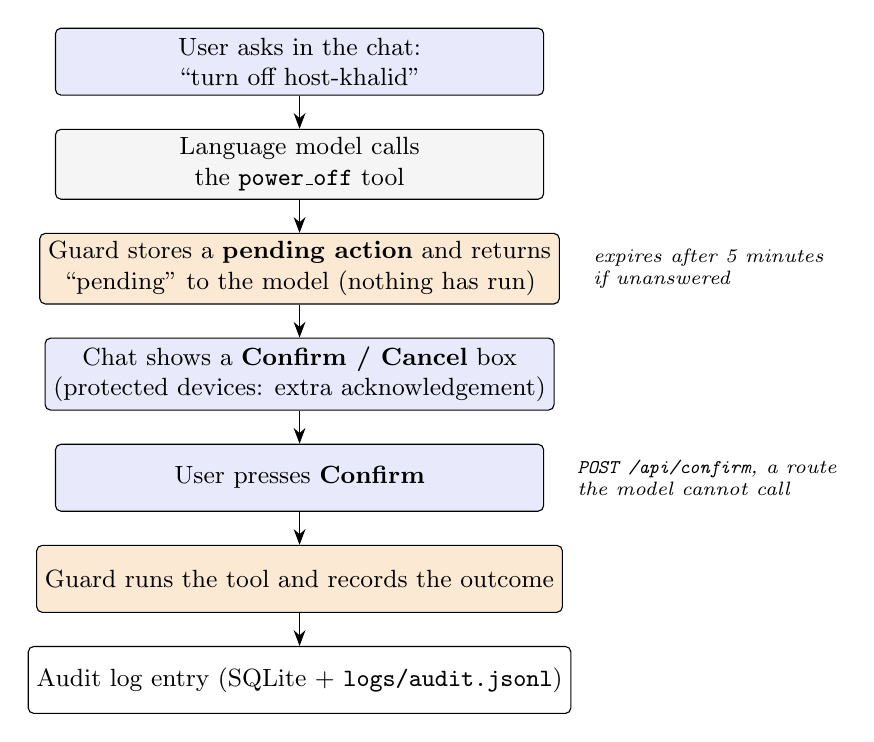
\begin{tikzpicture}[
  font=\small,
  stp/.style={draw,rounded corners=2pt,align=center,minimum width=6.2cm,minimum height=0.85cm,inner sep=3pt},
  user/.style={stp,fill=userblue},
  model/.style={stp,fill=boxgray},
  guard/.style={stp,fill=guardorange},
  side/.style={font=\scriptsize\itshape,align=left,anchor=west},
  >={Stealth[length=2mm]}, node distance=0.42cm]
  \node[user] (a) {User asks in the chat:\\``turn off host-khalid''};
  \node[model,below=of a] (b) {Language model calls\\the \code{power\_off} tool};
  \node[guard,below=of b] (c) {Guard stores a \textbf{pending action} and returns\\``pending'' to the model (nothing has run)};
  \node[user,below=of c] (d) {Chat shows a \textbf{Confirm / Cancel} box\\(protected devices: extra acknowledgement)};
  \node[user,below=of d] (e) {User presses \textbf{Confirm}};
  \node[guard,below=of e] (f) {Guard runs the tool and records the outcome};
  \node[stp,below=of f] (g) {Audit log entry (SQLite + \code{logs/audit.jsonl})};
  \foreach \x/\y in {a/b,b/c,c/d,d/e,e/f,f/g} \draw[->] (\x) -- (\y);
  \node[side] at ($(c.east)+(0.3,0)$) {expires after 5 minutes\\if unanswered};
  \node[side] at ($(e.east)+(0.3,0)$) {\code{POST /api/confirm}, a route\\the model cannot call};
\end{tikzpicture}
\caption{Confirmation flow for destructive actions: the model can only create a pending action; only the user's button press executes it}
\label{fig:confirm}
\end{figure}

% ------------------------------------------------------------
\subsection{Tool Registry, Network Backends and Model Provider}

In the first version, the model-facing description of every tool was written
by hand in the web server, and separate tables mapped tool names to functions
for each mode. The same information therefore lived in several places, and
the rule that real mode is read-only was only stated in the prompt. Following
the supervisor's assessment, this part of the system was refactored in
November into three small, independently tested pieces.

\textbf{Tool registry.} A tool is one plain Python function decorated with
the capability it needs and its risk level. The schema the model receives is
generated from the function itself: its name, its type hints, and the
parameter descriptions in its docstring. Adding a tool means writing one
function; nothing else lists tools. The simulated mode currently offers
seventeen tools, and the real mode three.

\textbf{Network backends.} The \code{NetworkBackend} interface describes a
network NetMind can talk to. \code{ContainerlabBackend} declares six
capabilities (inventory, segments, diagnostics, power, firewall and camera);
\code{RealLanBackend} declares only inventory. The set of tools offered to the
model in each mode is derived from the backend's capabilities, and calling a
tool whose capability the backend lacks raises an error in code. The
read-only guarantee for the real network (NFR4) therefore no longer depends
on the prompt. The same interface is also the extension point for future
backends, such as virtual machines or real network devices.

\textbf{Model provider.} The agent loop only calls one method,
\code{complete(messages, tools)}, on an \code{LLMProvider}. The Groq provider
implements it with an OpenAI-compatible client, so changing the model vendor
means writing one small class, which is what the model comparison planned for
Project 2 relies on. The Groq client and all settings are created on first
use rather than when the program is imported, so the application, and its
tests, start even without an API key or Docker.

% ------------------------------------------------------------
\subsection{Persistence and Least Privilege}

\textbf{Persistence.} Chat sessions, their messages, and the audit log are
stored in a SQLite database (\code{logs/netmind.db}), created readable by its
owner only because it contains chat text. One connection is shared by the
server's threads and guarded by a lock. A storage failure never breaks a
request: the agent catches it and carries on in memory. The alert history is
kept in \code{logs/alerts.json}, so a device that is down across a restart
keeps its original alert and its downtime keeps counting.

\textbf{Running without root.} The server needs exactly two privileges: a raw
socket for ARP scanning, and root rights to re-attach a lab device to its
bridge after power-on. Rather than running the whole server with
\code{sudo}, \code{make setup-perms} grants each one narrowly. A private copy
of the virtualenv's Python receives only the raw-socket capability
(\code{CAP\_NET\_RAW}), and \code{make run} uses it when present. Re-attaching
is done by one small, root-owned helper script, \code{netmind-reconnect},
which the user may run through \code{sudo} without a password and which
checks every argument (the container must belong to the lab, the bridge must
exist, and names may contain only safe characters) before doing anything.

% ------------------------------------------------------------
\subsection{Web API, Alerts and Notifications}

The backend exposes a small REST API, listed in Appendix~\ref{app:api}. The
chat endpoint runs the agent loop, bounded at five tool-calling rounds. The
dashboard uses read endpoints for devices, alerts, and logs, and a power
endpoint for the on/off buttons (turning on runs directly; turning off returns
a pending action that goes through the guard).

The first version of the dashboard polled the Docker daemon device by device,
which made one refresh take more than fifteen seconds with the full lab
running. Four changes made refreshes fast enough for regular polling:

\begin{enumerate}
\item all container states are read from a single container listing;
  per-container statistics, the slowest call and the only source of the CPU
  figures, are no longer requested, and the dashboard shows status rather than
  CPU usage;
\item the computed result is cached for three seconds, and concurrent callers
  share one computation instead of each starting their own;
\item firewall audits and camera credential checks used for the alert list
  are cached for ten seconds, and the cache is cleared whenever a rule,
  password or power state changes;
\item the frontend coalesces overlapping refreshes and releases a pressed
  button when its action finishes, so a button can no longer remain stuck.
\end{enumerate}

Three views sit on top of this state. The \emph{alert history} records a
``Device Offline'' alert when a device goes down and a ``Device Back Online''
alert, with the measured downtime, when it returns; the earlier alert is
closed but never deleted, so the history shows both that a device went down
and how long recovery took. Firewall findings and cameras still using their
default password raise alerts the same way, each stamped once with the time
it was first seen. The \emph{activity log} is built from the audit log and
lists the actions people and the assistant requested (power changes, port
changes, camera password changes), who requested them and how each one
ended: awaiting confirmation, confirmed, cancelled, denied or expired. A
\emph{report} view summarises open security findings, outages, average and
longest recovery time and operator activity, and can be printed or saved as a
PDF.

When a Telegram bot is configured, every alert and every recovery is also
sent as a message containing the network, the device, the event, its severity
and the time, and real-network devices joining or leaving the network are
reported the same way. A test button in the interface sends a test message,
so the setup can be checked in one click. The integration is optional: without
the two settings it does nothing, and a failure to send never breaks the
request that triggered it.

The web server accepts requests only from its own origin and listens on the
local machine only. A request carrying a different \code{Origin} header is
refused, so a web page open in the same browser cannot power a device off or
confirm a pending action through the user's session.

% ------------------------------------------------------------
\section{Verification and Testing}
\label{sec:testing}

Verification used four layers, summarised in Table~\ref{tab:verification}.

{\small
\begin{xltabular}{\textwidth}{|L{3.6cm}|Y|L{2.4cm}|}
\hline
\head \textbf{Layer} & \textbf{What it checks} & \textbf{Result} \\ \hline
\endhead
Unit and endpoint tests (pytest, 153 test functions in 17 files) & Argument parsing, session pruning and history trimming, the guard (pending, confirm, cancel, expiry, protected acknowledgement, password redaction), the retry safety net, the tool registry and generated schemas, backend capabilities, the services with a fake Docker layer, firewall rule parsing and rule application on both chains, SQLite storage, settings, the permission helper's argument checks, the merged real-network scan, API endpoints, and dashboard caching & All passing in CI, with test coverage of at least 70\% enforced \\ \hline
Browser UI tests (Playwright, 3 tests) & The real web server with a fake Docker layer, driven by a headless browser: powering a device off without its status flashing back online, the alert history, logs and report after an outage, and the chat view & Passing in CI \\ \hline
Integration test against the live lab (1 test) & A block rule on a firewall really stops traffic between branches, and the allow rule restores it & Passed on the team's lab \\ \hline
Manual browser verification & Pending, Confirm and Cancel flow, protected-device acknowledgement, audit log entries, power buttons after off/on, Arabic view, Real Network mode device list with \code{found\_by} & Passed \\ \hline
\caption{Verification layers and results}\label{tab:verification}\\
\end{xltabular}}

Static checks (ruff) and the pytest suite, with a minimum coverage of 70\%,
run automatically in GitHub Actions on every pull request. A dedicated test checks that the unit
tests cannot reach a Docker daemon at all, which proves that they run anywhere
without the lab or an API key. The integration test needs the
lab and is run on demand.

% ============================================================
\chapter{Conclusion}
% ============================================================

\section{Summary of Achievements}

NetMind set out to let someone responsible for a small or medium branch
network describe what they want in natural language, in either Arabic or
English, rather than learn a vendor-specific command-line syntax. By the end
of Project 1, both of the system's operating modes were working and
demonstrated: a simulated mode that queries and controls a real Containerlab
network of routers, firewalls, hosts, and cameras, and a read-only
real-network mode that discovers devices on the physical local network by
combining four discovery methods, without altering them. Destructive actions
are guarded by a confirmation step, protected devices need an extra
acknowledgement, and every outcome is written to an audit log. A live
dashboard, an alert history with Telegram notifications, persistent storage,
and an automated test suite running on every change complete the system. In
a pilot evaluation of 28 English and Arabic requests (Section~\ref{sec:pilot}),
the model behaved correctly in 27 cases, answered every request in the
language it was asked in, and no destructive action ran without the user's
confirmation.

Because development started early, the team also completed the first three
milestones of the supervisor's improvement plan within this term:
stabilisation (October), the architecture refactor (November) and, ahead of
its December target, observability, which added a background collector and
diagnostic and alert-history tools for the agent.
Figure~\ref{fig:scope} places what was actually built against what remains
for Project 2, and Table~\ref{tab:coverage} summarises, capability area by
capability area, how the requirements gathered in Chapter~3 were met.

\begin{figure}[H]
\centering
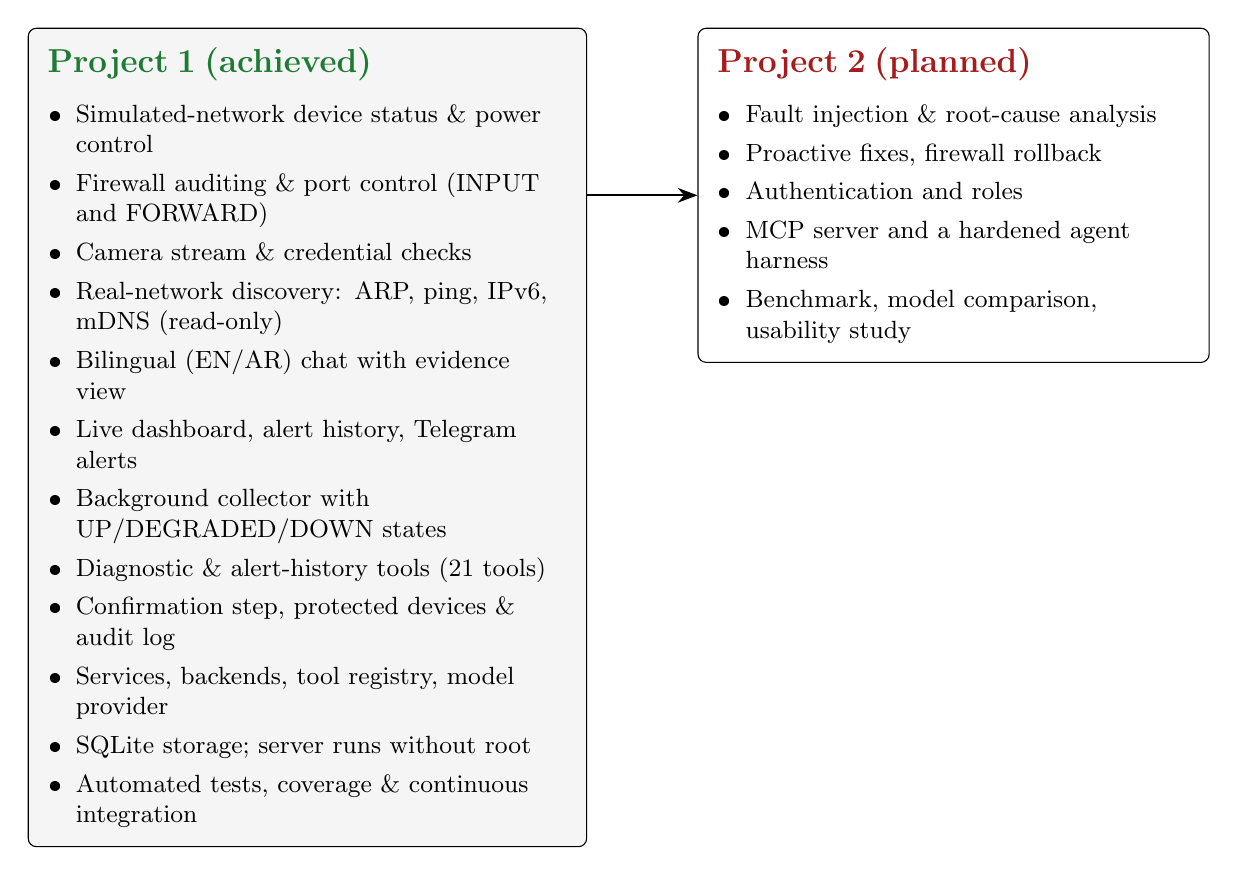
\begin{tikzpicture}[font=\small,>={Stealth[length=2.5mm]}]
  \node[draw,rounded corners=3pt,fill=boxgray,text width=6.6cm,inner sep=7pt,align=left] (p1) {%
    {\large\bfseries\color{donegreen}Project 1 (achieved)}\par\smallskip
    \begin{itemize}[leftmargin=1.1em,itemsep=1pt,topsep=2pt]
      \item Simulated-network device status \& power control
      \item Firewall auditing \& port control (INPUT and FORWARD)
      \item Camera stream \& credential checks
      \item Real-network discovery: ARP, ping, IPv6, mDNS (read-only)
      \item Bilingual (EN/AR) chat with evidence view
      \item Live dashboard, alert history, Telegram alerts
      \item Background collector with UP/DEGRADED/DOWN states
      \item Diagnostic \& alert-history tools (21 tools)
      \item Confirmation step, protected devices \& audit log
      \item Services, backends, tool registry, model provider
      \item SQLite storage; server runs without root
      \item Automated tests, coverage \& continuous integration
    \end{itemize}};
  \node[draw,rounded corners=3pt,text width=6.0cm,inner sep=7pt,align=left,right=1.4cm of p1.north east,anchor=north west] (p2) {%
    {\large\bfseries\color{nextred}Project 2 (planned)}\par\smallskip
    \begin{itemize}[leftmargin=1.1em,itemsep=1pt,topsep=2pt]
      \item Fault injection \& root-cause analysis
      \item Proactive fixes, firewall rollback
      \item Authentication and roles
      \item MCP server and a hardened agent harness
      \item Benchmark, model comparison, usability study
    \end{itemize}};
  \draw[->,thick] (p1.east |- p2.west) -- (p2.west);
\end{tikzpicture}
\caption{Project 1 (achieved) scope against Project 2 (planned) scope}
\label{fig:scope}
\end{figure}

{\small
\begin{xltabular}{\textwidth}{|Y|L{3.4cm}|}
\hline
\head \textbf{Capability Area} & \textbf{Status} \\ \hline
\endhead
Device status \& power control (FR1, FR2) & Met \\ \hline
Network/segment visibility (FR3) & Met \\ \hline
Firewall auditing \& port control (FR4, FR5) & Met \\ \hline
Camera stream \& credential checks (FR6) & Met \\ \hline
Real-network discovery, read-only (FR7, NFR4) & Met \\ \hline
Bilingual Arabic/English interface (FR8) & Met \\ \hline
Scope guarding: refusing unrelated requests (FR9) & Met \\ \hline
Live monitoring dashboard (FR10) & Met \\ \hline
Confirmation before destructive actions, protected devices, audit log (FR11--FR13, NFR6) & Met \\ \hline
Connectivity check between lab devices (FR14) & Met \\ \hline
Alert notifications outside the browser (FR15) & Met \\ \hline
Usability, performance, portability (NFR1--NFR3, NFR9--NFR13) & Met \\ \hline
Least privilege, persistence, automated checks (NFR8, NFR14, NFR15) & Met \\ \hline
Agent behaviour in the pilot evaluation (Table~\ref{tab:pilot}) & 27/28 correct; 0 unconfirmed actions \\ \hline
Authentication (NFR7) & Planned for Project 2 \\ \hline
\caption{Requirement coverage summary}\label{tab:coverage}\\
\end{xltabular}}

\section{Limitations}

Three limitations were deliberately accepted in Project 1 rather than left
unnoticed. The first is that the web interface does not yet authenticate its
users (NFR7). The server only listens on the local machine and refuses
requests from other origins, which keeps it safe on a single laptop, but it
assumes one trusted operator.

The second is an architectural trade-off described in Chapter~3: device state
such as power status, firewall rules, and camera credentials is read live from
Docker rather than stored in a database of NetMind's own. Only very short
caches are used (three seconds for the device list, ten seconds for audits),
and they are cleared whenever a power state, rule or password changes, so
NetMind's picture cannot drift from the lab. This means every query needs a
reachable Docker daemon and live containers, which is acceptable for a
lab-scale deployment but would need to be revisited if NetMind were ever
asked to manage a larger or longer-lived network.

The third is that the agent's accuracy has only been measured on a small
scale. The pilot evaluation in Section~\ref{sec:pilot} used 28 prompts, one
run and one model; it gives encouraging results but cannot show how
consistent the model is across runs or how it compares with others. The same
pilot showed a median response time of about 9.5~seconds, which is longer
than intended and not yet broken down into model and tool time.

Two limitations listed earlier have since been resolved: conversation
history, once held only in memory and lost on restart, is now kept in the
SQLite storage described in Chapter~5, and alerts, once computed only while
the dashboard was open, are now raised by the background collector.

{\small
\begin{xltabular}{\textwidth}{|Y|Y|}
\hline
\head \textbf{Limitation} & \textbf{Planned Resolution} \\ \hline
\endhead
No authentication on the web interface & Authentication with viewer, operator and admin roles (\#31) \\ \hline
Device state read live from Docker & Kept for the lab; storing metrics over time is a possible extension \\ \hline
Accuracy measured only in a 28-prompt pilot; slow replies & Prompt benchmark with repeated runs, model comparison, latency breakdown and usability study (\#34--\#38) \\ \hline
\caption{Limitations and their planned resolution}\label{tab:limitations}\\
\end{xltabular}}

\section{Future Work}

Project 2 continues the supervisor's seven-month plan, which is tracked as
GitHub issues (issue numbers are given in brackets). Milestones M1 to M3 were
completed this term; the remaining milestones, adjusted to the academic
calendar, are listed in Table~\ref{tab:roadmap}.

{\small
\begin{xltabular}{\textwidth}{|L{3.4cm}|Y|}
\hline
\head \textbf{Milestone} & \textbf{Planned Work} \\ \hline
\endhead
M4: Diagnosis & Reversible fault-injection scenarios such as a link going down, packet loss, a stopped service or a firewall misconfiguration (\#25); root-cause-analysis playbooks that diagnose a fault step by step with evidence (\#26) \\ \hline
M5: Safe change & Proactive suggestions and remediation playbooks, always through the confirmation flow (\#29); firewall snapshots, diff, dry run and rollback (\#30); authentication and roles (\#31); new-device detection on the real network (\#32) \\ \hline
M6: Evaluation & A benchmark of more than 100 English and Arabic prompts measuring tool-selection accuracy, latency and safety (\#34, \#38); comparison of LLM providers and models (\#35); failure and load testing (\#36); a usability study (\#37) \\ \hline
M7: Delivery & Final thesis chapters, a v1.0 release, demo and mock defences (\#39--\#41) \\ \hline
\caption{Project 2 milestones}\label{tab:roadmap}\\
\end{xltabular}}

In addition to the plan, two pieces of work suggested by the supervisor
build directly on the structure delivered this term.

\textbf{An MCP server.} The Model Context Protocol (MCP) is an open standard
through which AI assistants connect to external tools. NetMind's tools
already exist as registered functions with generated schemas, capabilities
and risk levels, so they can be published through an MCP server. Any
MCP-compatible assistant could then query and manage the lab through the same
safety guard, confirmation flow and audit log, rather than only through
NetMind's own chat.

\textbf{A hardened agent harness.} The harness is the program around the
model that runs the loop: it sends the request, lets the model call a tool,
checks and runs the call, feeds the result back, and decides when to stop.
NetMind's agent loop is already a small harness with a round limit, a retry
safety net and a guard. Project 2 will strengthen it with clearer limits and
timeouts, structured logging of every step, and the prompt benchmark above,
so that changes to the model, the prompt or the tools can be measured rather
than judged by eye.

Figure~\ref{fig:timeline} places Project 1's phases on a timeline, for
reference against the Project 2 work that follows it.

\begin{figure}[H]
\centering
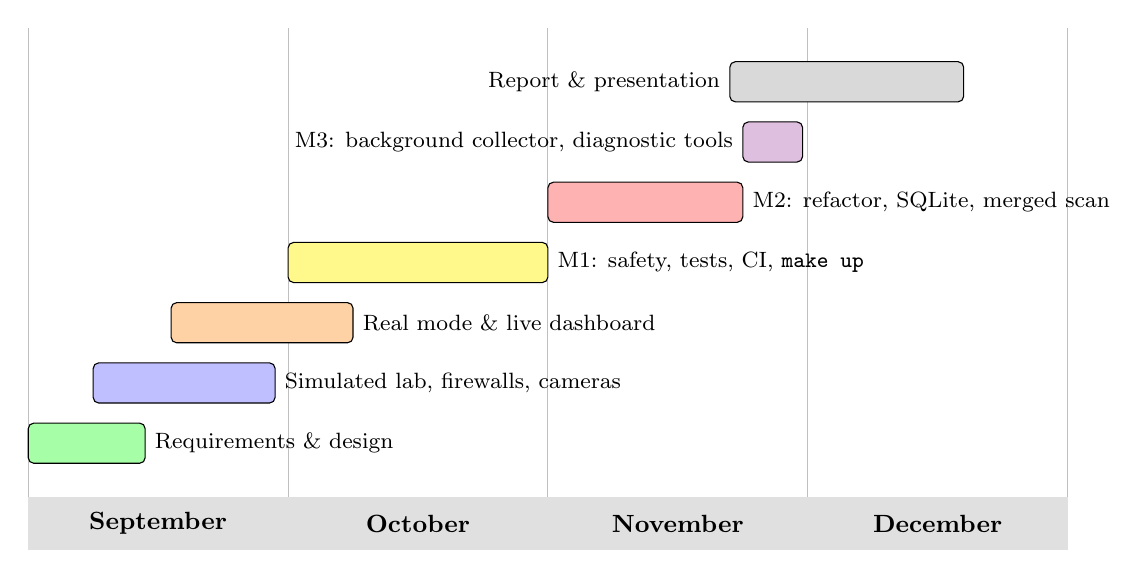
\begin{tikzpicture}[font=\footnotesize,x=3.3cm,y=0.85cm]
  \foreach \m/\i in {September/0,October/1,November/2,December/3}{
    \fill[headgray] (\i,0) rectangle (\i+1,-0.8);
    \node[font=\small\bfseries] at (\i+0.5,-0.4) {\m};
    \draw[black!25] (\i,0) -- (\i,7.0);
  }
  \draw[black!25] (4,0) -- (4,7.0);
  % \ph{start}{end}{row}{colour}{text}  (x in months from 1 September)
  % \ph{start}{end}{row}{colour}{text}: bar in months from 1 September, label to its right
  \newcommand{\ph}[5]{\draw[rounded corners=2pt,fill=#4] (#1,#3-0.3) rectangle (#2,#3+0.3);
    \node[anchor=west,font=\footnotesize] at (#2,#3) {#5};}
  \ph{0.0}{0.45}{0.8}{green!35}{Requirements \& design}
  \ph{0.25}{0.95}{1.7}{blue!25}{Simulated lab, firewalls, cameras}
  \ph{0.55}{1.25}{2.6}{orange!35}{Real mode \& live dashboard}
  \ph{1.0}{2.0}{3.5}{yellow!45}{M1: safety, tests, CI, \code{make up}}
  \ph{2.0}{2.75}{4.4}{red!30}{M2: refactor, SQLite, merged scan}
  \draw[rounded corners=2pt,fill=violet!25] (2.75,5.0) rectangle (2.98,5.6);
  \node[anchor=east,font=\footnotesize] at (2.75,5.3) {M3: background collector, diagnostic tools};
  \draw[rounded corners=2pt,fill=black!15] (2.7,5.9) rectangle (3.6,6.5);
  \node[anchor=east,font=\footnotesize] at (2.7,6.2) {Report \& presentation};
\end{tikzpicture}
\caption{Project 1 timeline, by phase}
\label{fig:timeline}
\end{figure}

Taken together, Project 1 delivered a working, demonstrated system covering
both of NetMind's operating modes, together with the safety, storage and
testing foundations that the planned work depends on. The remaining work is
to make NetMind diagnose faults, change the network safely, and measure how
well it does so; it extends what already exists
rather than redesigning it.


% ============================================================
% References (APA 7th edition), entered by hand
% ============================================================
\cleardoublepage
\chapter*{REFERENCES}
\addcontentsline{toc}{chapter}{REFERENCES}

\begin{list}{}{%
  \setlength{\leftmargin}{2.2em}%
  \setlength{\itemindent}{-2.2em}%
  \setlength{\itemsep}{0.6em}%
  \setlength{\parsep}{0pt}}
\raggedright

\item Anthropic. (2024). \textit{Model Context Protocol specification}.
Retrieved November 23, 2026, from \url{https://modelcontextprotocol.io}

\item Hong, J., Van Tu, N., \& Hong, J. W.-K. (2025). A comprehensive survey
on LLM-based network management and operations. \textit{International Journal
of Network Management, 35}(6), Article e70029.
\url{https://doi.org/10.1002/nem.70029}

\item Jiang, X., Gember-Jacobson, A., \& Feamster, N. (2024). CAIP: Detecting
router misconfigurations with context-aware iterative prompting of LLMs.
\textit{arXiv}. \url{https://doi.org/10.48550/arXiv.2411.14283}

\item Lorusso, R., Maci, A., \& Coscia, A. (2025). GOLLUM: Guiding
cOnfiguration of firewaLL through aUgmented large language Models. In
\textit{Proceedings of the 17th International Conference on Agents and
Artificial Intelligence (ICAART 2025) -- Volume 1} (pp.~489--496).
SciTePress. \url{https://doi.org/10.5220/0013221900003890}

\item ntunes. (n.d.). \textit{JACE: Autonomous control engine} [Computer
software]. GitHub. Retrieved October 3, 2026, from
\url{https://github.com/ntunes/jace}

\item Selector AI. (n.d.). \textit{Network LLM \& Copilot}. Retrieved October
3, 2026, from \url{https://www.selector.ai/network-llm-copilot/}

\item Wang, Z., Lin, S., Yan, G., Ghorbani, S., Yu, M., Zhou, J., Hu, N.,
Baruah, L., Peters, S., Kamath, S., Yang, J., \& Zhang, Y. (2025).
Intent-driven network management with multi-agent LLMs: The Confucius
framework. In \textit{Proceedings of the ACM SIGCOMM 2025 Conference}
(pp.~347--362). Association for Computing Machinery.
\url{https://doi.org/10.1145/3718958.3750537}

\end{list}


\appendix
\titleformat{\chapter}[block]
  {\normalfont\LARGE\bfseries}
  {APPENDIX \thechapter:\ }{0pt}{\MakeUppercase}
% ============================================================
\chapter{REST API}
\label{app:api}
% ============================================================

Table~\ref{tab:api} lists the endpoints exposed by the NetMind backend. The
destructive actions reachable through the chat or the power endpoint produce
pending actions; only \code{/api/confirm} executes them, and it is called by
the interface, never by the language model. The server listens on
\code{127.0.0.1} and refuses requests from other origins.

{\small
\begin{xltabular}{\textwidth}{|L{5.4cm}|Y|}
\hline
\head \textbf{Method and path} & \textbf{Purpose} \\ \hline
\endhead
\code{POST /api/chat} & Run the agent loop for one user message; returns the reply, mode, evidence steps, and any pending actions \\ \hline
\code{POST /api/confirm} & Confirm or cancel a pending action (called by the interface only) \\ \hline
\code{GET /api/pending} & List pending actions \\ \hline
\code{GET /api/audit} & Audit log entries \\ \hline
\code{GET /api/devices} & Simulated devices with id, type, IP address, branch and status \\ \hline
\code{GET /api/alerts} & Alert history, newest first: devices going offline, degraded and back online (with downtime), firewall and camera findings \\ \hline
\code{POST /api/alerts/\{id\}/ack} & Acknowledge an alert (records that an operator has seen it; it stays open until the device recovers) \\ \hline
\code{GET /api/health} & The background collector's status and each device's confirmed state (up, degraded or down) \\ \hline
\code{GET /api/events} & Server-sent event stream telling the dashboard when alerts or device states change \\ \hline
\code{GET /api/logs} & Activity log: requested and confirmed actions, who made them, and their outcome \\ \hline
\code{GET /api/report} & Security and reliability summary \\ \hline
\code{POST /api/devices/\{id\}/power} & Turn a device on (runs) or off (creates a pending action) \\ \hline
\code{POST /api/notify-test} & Send a Telegram test message, if Telegram is configured \\ \hline
\code{GET /api/real-devices} & Real-network devices with IPv4, IPv6, MAC, hostname, status and \code{found\_by} (read-only) \\ \hline
\code{GET /api/real-alerts}, \code{/api/real-logs} & Real Network mode counterparts: alerts, and devices joining or leaving the network \\ \hline
\caption{REST API endpoints}\label{tab:api}\\
\end{xltabular}}

% ============================================================
\chapter{Running NetMind}
% ============================================================

From the repository root, inside WSL2 Ubuntu with a native docker-ce engine
and Containerlab installed:

\begin{enumerate}
\item Create a virtual environment and install the dependencies with
  \code{pip install -r requirements.txt}. Add \code{GROQ\_API\_KEY} to a
  \code{.env} file, and optionally \code{TELEGRAM\_BOT\_TOKEN} and
  \code{TELEGRAM\_CHAT\_ID} for notifications.
\item \code{make setup-perms} (once) gives the server the raw-socket
  capability and the re-attach helper, so it does not need to run as root.
\item \code{make up} builds the images, creates the Linux bridges, deploys the
  lab, and writes \code{registry.json}.
\item \code{make run} starts the web server, reachable at
  \code{http://127.0.0.1:8000}.
\item \code{make test} runs the automated tests, and \code{make lint} runs ruff.
\item \code{make down} removes the lab.
\end{enumerate}

% ============================================================
\chapter{Design Details}
\label{app:design}
% ============================================================

This appendix gives the detailed reasoning behind two parts of the design
that Chapter~5 summarises.

\section{Real-Network Discovery: Design Decisions}
\label{app:scan}

The decisions below are summarised in Table~\ref{tab:decisions}.

\textbf{Subnet detection.} The active interface is found by opening a UDP
socket towards a public address and reading the local address the operating
system assigns to it. No packet is actually sent, and the method relies only
on the Python standard library. If there is no default route at all, the
module reads the interface configuration with \code{ip addr} instead.
Alternatives were the netifaces and psutil libraries, which are more accurate
on machines with several interfaces but add an external dependency, and
gethostbyname applied to the machine's own hostname, which frequently returns
the loopback address 127.0.0.1 and is therefore unreliable. The chosen method
assumes a /24 subnet, which is a known limitation.

\textbf{Host discovery with ARP, Scapy and a ping sweep.} ARP was chosen
because it works at the data link layer: a device cannot ignore an ARP
request and still take part in an Ethernet network, so ARP finds devices that
are configured to block ICMP ping, and it also returns the MAC address. Scapy
was chosen to send the requests because it is a pure Python library that
integrates directly with the rest of the code and gives full control over
packet construction without an external program. In practice, however, some
devices answer ping but miss the short ARP window, so the ping sweep is not
only a fallback: running both and merging the results finds more devices than
either method alone, and \code{found\_by} makes visible which method saw each
device. The alternatives were Nmap, used directly or through python-nmap,
which is far more capable but is a separate binary larger than this module
requires; the arp-scan command-line tool, which is fast but is again an
external dependency; the operating system's ARP cache, which only lists
devices that the machine has already communicated with; and passive sniffing
of network traffic, which needs no probes but can take a long time to reveal
quiet devices.

\textbf{IPv6.} An IPv6 subnet is far too large to sweep, so the module sends
one ping to the IPv6 all-nodes multicast address on the active interface. Every
IPv6 device on the link answers, which places it in the kernel's neighbour
table; the module then reads that table and attaches each IPv6 address to the
device with the same MAC address. A device often has several IPv6 addresses
(a link-local \code{fe80::} address and one or more global ones), and all are
listed.

\textbf{Concurrency.} Checking 254 addresses one after another would take
several minutes, since each unanswered ping waits up to one second. A
ThreadPoolExecutor with 64 workers runs the pings in parallel and reduces the
sweep to a few seconds, and a second small pool runs the four discovery
methods at the same time, so a full scan takes about as long as its slowest
method. Threads suit this task because it is bound by waiting on the network
rather than by computation. The alternatives were multiprocessing, whose
separate processes add memory and start-up cost for work that is only
waiting, and asyncio, which would be efficient but would require the
surrounding code to be restructured around asynchronous functions.

\textbf{Hostname discovery with mDNS.} Multicast DNS was chosen because small
and home networks often have no reverse DNS records, so a reverse lookup
alone returns no name for most devices. mDNS lets printers, AirPlay devices,
Chromecast devices, and shared workstations announce their names without any
credentials or access to the router, and the zeroconf library provides a pure
Python implementation. The browse runs on every scan rather than once at
server start, so that a device that joins the network later is still found.
The alternatives were NetBIOS name queries, which are mostly limited to
Windows hosts; SSDP and UPnP discovery, which cover fewer device types; DHCP
lease tables read from the router, which need administrative access to the
router; and SNMP queries, which need SNMP to be enabled and credentials to be
known. A limitation of mDNS is that a device which advertises no service, such
as an idle phone, appears without a hostname, although it is still listed by
IP and MAC address.

\textbf{Reverse DNS and status checking.} Reverse DNS through the standard
library is used as a secondary source, because it is already available in
Python at no cost and gives names on networks that do maintain DNS records.
The status of a single device is determined with one ping, which keeps it
consistent with the ping sweep and needs no extra dependency. A TCP
connection check or an ARP probe would be more reliable against devices that
block ICMP, and are identified as possible improvements.

\textbf{Optional dependencies and output format.} Scapy and zeroconf are
imported inside try and except blocks, and their availability is recorded in
flags. If either library is missing the module degrades gracefully instead of
failing to start, which makes it easier to run on different machines. Results
are returned as plain dictionaries, rather than custom classes, because they
map directly to JSON for the API.

\section{Dashboard Refresh Performance}
\label{app:dash}

The first version of the dashboard polled the Docker daemon device by device,
which made one refresh take more than fifteen seconds with the full lab
running. Four changes made refreshes fast enough for regular polling:

\begin{enumerate}
\item all container states are read from a single container listing;
  per-container statistics, the slowest call and the only source of the CPU
  figures, are no longer requested, and the dashboard shows status rather than
  CPU usage;
\item the computed result is cached for three seconds, and concurrent callers
  share one computation instead of each starting their own;
\item firewall audits and camera credential checks used for the alert list
  are cached for ten seconds, and the cache is cleared whenever a rule,
  password or power state changes;
\item the frontend coalesces overlapping refreshes and releases a pressed
  button when its action finishes, so a button can no longer remain stuck.
\end{enumerate}


\end{document}
